\documentclass{itor}
\usepackage[authoryear]{natbib}
\usepackage[T1]{fontenc}
\usepackage[utf8]{inputenc}
\usepackage{amsmath,amssymb,amsthm}
\usepackage{physics}
\usepackage{graphicx}
\usepackage{booktabs,multirow}
\usepackage{xcolor}
\usepackage{placeins,float}
\usepackage{algorithm}
\usepackage{algpseudocode}
\usepackage{subcaption}
\usepackage{caption}
\usepackage{hyperref}
\usepackage{cleveref}
\newtheorem{proposition}{Proposition}

\jvol{}
\jyear{}
\doi{}

\begin{document}
\title{A risk-averse two-stage stochastic firebreak placement problem:
Graph-based valid inequalities and exact decomposition}

\author[Quezada et al.]{Franco Quezada\affmark{a,b,$\ast$}, Mat\'ias Vilches\affmark{a}, Sebasti\'an D\'avila-G\'alvez\affmark{a,b} and Jaime Carrasco\affmark{c,d}}

\affil{\affmark{a}Industrial Engineering Department, Faculty of Engineering, University of Santiago of Chile, Santiago, Chile}
\affil{\affmark{b}Program for the Development of Sustainable Production Systems, Faculty of Engineering, University of Santiago of Chile, Santiago, Chile}
\affil{\affmark{c}Departamento de Industria, Facultad de Ingenier\'ia, Universidad Tecnol\'ogica Metropolitana, Santiago, Chile}
\affil{\affmark{d}Complex Engineering Systems Institute -- ISCI, Santiago, Chile}
\email{franco.quezada@usach.cl [F. Quezada];matias.vilches.a@usach.cl [M. Vilches];\\ sebastian.davila@usach.cl [S. D\'avila-G\'alvez]; jcarrascob@utem.cl [J. Carrasco]}
\thanks{\affmark{$\ast$}Corresponding author: franco.quezada@usach.cl.}

\begin{abstract}
Firebreak placement must account for uncertainty in wildfire ignition and propagation and the consequences of extreme events. We formulate the Firebreak Placement Problem as a risk-averse two-stage stochastic program minimizing a weighted combination of expected loss and Conditional Value-at-Risk (CVaR). Wildfire scenarios from Cell2Fire are represented by directed propagation graphs. We develop an exact Branch-and-Benders decomposition framework strengthened by two families of graph-based valid inequalities exploiting downstream coverage and propagation paths. We prove their validity for general directed graphs and show that the complete path-based family characterizes the linear programming recourse function under fractional firebreak decisions. Experiments on 810 instances show that the path-strengthened algorithm achieves an optimality certification rate of 84.9\%, compared with 77.3\% for a combinatorial Branch-and-Benders benchmark and 63.6\% for the extensive mixed-integer formulation. Its advantages are strongest under risk-sensitive objectives, while the combinatorial benchmark is faster for expected-loss minimization. 
\end{abstract}
\keywords{Firebreak placement; Two-stage stochastic programming; Conditional Value-at-Risk; Branch-and-Benders decomposition; Graph-based valid inequalities}
\maketitle

\section{Introduction}
\label{sec1}

Wildfires pose substantial threats to ecosystems, biodiversity,
and human communities. Their increasing frequency and severity,
together with more favorable fire-weather conditions associated
with climate change, have intensified concerns about their
environmental and socioeconomic consequences
\citep{jones2020climate,westerling2016increasing}.
Large wildfire events can cause extensive biodiversity losses
\citep{keeley2019fire,kelly2020fire,miranda2023widespread}
and adversely affect human health through smoke exposure
and associated environmental impacts
\citep{delfino2009relationship,dennekamp2011effects,
johnston2009bushfires,johnston2012estimated}.
These challenges highlight the importance of complementing
fire suppression with preventive strategies aimed at reducing
the consequences of future wildfires.

Among preventive measures, firebreaks seek to interrupt wildfire
propagation by removing or modifying vegetation along selected
areas of a landscape. Together with natural barriers, they
can influence fire behavior and limit the extent of wildfire
spread \citep{agee2000use}. Previous studies have shown that
vegetation management and landscape configuration can
substantially affect wildfire propagation patterns
\citep{amiro2001fire,kim2009spatial,cheney1993influence,
carrasco2023firebreak}. However, establishing firebreaks
involves considerable intervention costs, and only a limited
portion of a landscape can generally be treated
\citep{oliveira2016assessing}. Consequently, determining
where to place firebreaks is a critical planning decision,
whose effectiveness depends not only on the selected
locations but also on how future fires propagate
through the landscape.

Operations Research has addressed wildfire prevention and
management through various optimization approaches
\citep{martell2007forest,ronnqvist2015operations}.
Early studies incorporated simplified representations of
fire ignition and propagation into spatially explicit
integer and dynamic programming models
\citep{bettinger2009,kim2009spatial,konoshima2008spatial,
gonzalez2011integrating}. Other approaches introduced
stochastic optimization to account for uncertainty in
wildfire occurrence and behavior. For instance,
\citet{boychuk1996multistage} developed a multistage
stochastic programming model incorporating wildfire risk
into forest planning, whereas \citet{kabli2015stochastic}
proposed a two-stage stochastic formulation for fuel
treatment decisions. These developments established the
relevance of incorporating uncertainty into forest
management, although representing the spatial interactions
between firebreak placement and wildfire propagation
remains challenging.

Another important line of research relies on wildfire
simulation to characterize spatial exposure through
burn probability (BP) maps. These maps estimate the
probability that a given landscape cell will burn,
typically using repeated simulations of wildfire
ignition and propagation
\citep{parisien2005mapping,finney2005challenge}.
Simulation tools such as FARSITE \citep{finney1998farsite},
Burn-P3 \citep{parisien2005mapping}, and Cell2Fire
\citep{pais2021cell2fire} provide spatially explicit
representations of wildfire behavior. Burn probability
estimates have been used to support preventive management
decisions by identifying areas with high exposure
\citep{ager2010comparison,oliveira2016assessing}.
Nevertheless, marginal burn probabilities do not directly
describe how a specific firebreak configuration modifies
the connectivity of wildfire propagation networks.
In particular, they do not explicitly capture the
interactions between treatments located along different
propagation paths. Moreover, uncertainty in burn
probability estimates introduces additional challenges
when interpreting these measures
\citep{kuhlmann2015generating}.

Recent research has therefore increasingly considered
graph-based representations of wildfire propagation
within optimization models. For example,
\citet{yemshanov2025graph} developed a network optimization
framework that represents wildfire spread through
directed propagation graphs and evaluates alternative
firebreak allocation strategies. Their formulations
incorporate treatment budgets, spatial contiguity
requirements, and different representations of fire
propagation across interconnected landscape cells.
Such approaches demonstrate the value of explicitly
accounting for propagation structure when optimizing
firebreak placement. Related methodological advances have been developed
in stochastic network optimization. In particular,
\citet{taninmics2024benders} studied the Measure-Based
Spread Minimization Problem and proposed exact
Branch-and-Benders-cut algorithms based on arc- and
path-based formulations. Their work demonstrates how
the structure of stochastic propagation networks can
be exploited to develop combinatorial procedures for
generating optimality cuts. These algorithms provide
an important methodological benchmark for the
development of exact decomposition approaches to
firebreak placement.

Despite these advances, two important challenges
remain. First, the uncertain nature of wildfire
propagation makes it necessary to consider not only
average losses but also the potentially severe
consequences of adverse wildfire scenarios.
Firebreak configurations that perform well on average
may provide insufficient protection against extreme
events, motivating the integration of risk measures
into stochastic firebreak placement models. Second,
the resulting optimization problems are computationally
challenging. Extensive mixed-integer formulations
introduce scenario-dependent variables and constraints
to represent wildfire propagation, and their size
increases with the number of scenarios. Although
decomposition offers a natural alternative by
separating firebreak placement decisions from
scenario-dependent loss evaluation, its effectiveness
depends on obtaining sufficiently strong approximations
of the recourse function. This is particularly
challenging in propagation graphs containing multiple
paths between ignition points and affected cells,
where the protection associated with an individual
firebreak may depend on alternative routes through
the network.

Motivated by these challenges, this paper develops
a risk-averse stochastic programming approach to
the Firebreak Placement Problem (FPP), together with
an exact decomposition method that exploits wildfire
propagation structure. We consider spatially explicit
wildfire scenarios represented by directed propagation
graphs and formulate firebreak placement as a two-stage
stochastic optimization problem. The objective combines
expected wildfire losses with Conditional Value-at-Risk
(CVaR), allowing different levels of emphasis on
average and adverse wildfire outcomes.

The contributions of this paper are twofold. First, we develop a risk-averse two-stage stochastic
programming framework for the FPP that explicitly
accounts for uncertainty in wildfire ignition and
propagation. Wildfire behavior is represented through
spatially explicit scenarios generated by a fire
spread simulator, allowing firebreak placement
decisions to be evaluated across different propagation
patterns. By incorporating CVaR into the objective,
the proposed formulation accounts for the potentially
severe consequences of adverse wildfire scenarios.
Combining expected loss and CVaR within a unified
optimization framework enables decision-makers to
examine the trade-off between reducing average
wildfire impacts and limiting exposure to extreme
outcomes. Second, we develop an exact Branch-and-Benders
decomposition framework strengthened by graph-based
valid inequalities that exploit the structure of
wildfire propagation networks. We derive two
complementary families of inequalities based on
downstream coverage and directed propagation paths,
providing lower bounds on scenario-dependent
recourse costs. We establish their validity for
general directed propagation graphs and show that
the complete family of path-based inequalities
characterizes the linear programming recourse
function over fractional firebreak decisions.
We further develop separation procedures to
incorporate these inequalities into the decomposition
framework, strengthening the approximation of
scenario recourse within the master problem.
Extensive computational experiments demonstrate
that the resulting path-based algorithm outperforms
both the extensive MILP formulation and a
state-of-the-art combinatorial Branch-and-Benders
algorithm for stochastic network spread minimization,
adapted from \citet{taninmics2024benders}, in
terms of overall computational performance. Computational results demonstrate that the proposed
decomposition approach outperforms both the extensive
MILP formulation and a state-of-the-art combinatorial
Branch-and-Benders algorithm in overall computational
performance, with particularly pronounced advantages
under risk-averse objectives.

The remainder of this paper is organized as follows.
Section~\ref{sec2} introduces the problem setting
and the relevant theoretical background.
Section~\ref{s:general-model} presents the two-stage
stochastic programming formulation. Section~4
develops the Branch-and-Benders decomposition
framework and the graph-based valid inequalities.
Section~\ref{sec:computational} presents the
computational experiments and discusses algorithmic
performance and out-of-sample solution quality.
Finally, Section~\ref{sec:conclusions} summarizes
the main findings and discusses directions for
future research.


\section{Problem setting and risk measures}
\label{sec2}

We first describe the landscape representation, wildfire
scenarios, and feasible firebreak placement decisions.
We then introduce the expected-loss and risk measures
used to evaluate these decisions.

\subsection{Landscape and wildfire scenarios}

The landscape is represented by a graph
$\mathcal{F}=(\mathcal{V},\mathcal{E})$, where
$\mathcal{V}$ denotes the set of landscape cells and
$\mathcal{E}$ represents their spatial adjacency.
The discretization is determined by georeferenced
landscape data, including vegetation, elevation, slope,
and aspect. We consider an eight-neighbor grid, in
which each cell may be adjacent to its horizontal,
vertical, and diagonal neighbors. Each cell
$v\in\mathcal{V}$ is assigned a nonnegative weight
$w_v$, representing its relative value or protection
priority. These weights allow the model to account
for differences in the importance of landscape
cells \citep{carrasco2023firebreak}.

Wildfire uncertainty arises from two interconnected
processes: ignition and propagation. Ignition locations
may follow spatial probability distributions that reflect
natural or human-related ignition patterns
\citep{carrasco2021exploring}. In this study, ignition
locations are sampled uniformly across the landscape.
Wildfire propagation is simulated using Cell2Fire
\citep{pais2021cell2fire}, which accounts for the
influence of landscape characteristics and
environmental conditions on fire spread.

Let $\Omega$ denote a finite set of wildfire scenarios,
indexed by $\omega$. Each scenario is associated with
an ignition cell $v(\omega)\in\mathcal{V}$ and a
directed propagation graph
$\mathcal{T}^{\omega}
=(\mathcal{V}^{\omega},\mathcal{E}^{\omega})$.
The set $\mathcal{V}^{\omega}\subseteq\mathcal{V}$
contains the cells reached by the simulated wildfire
in the absence of firebreaks, while
$\mathcal{E}^{\omega}$ represents the directed
propagation connections between these cells.
These connections are obtained from the information
recorded during the wildfire simulation
\citep{pais2021downstream}. For each $v\in\mathcal{V}^{\omega}$, let 
$\delta_+^{\omega}(v)
=
\{u\in\mathcal{V}^{\omega}:
(v,u)\in\mathcal{E}^{\omega}\}$ 
denote its set of outgoing neighbors.
The propagation graphs may contain multiple
directed paths connecting the ignition cell to
a given destination. The mathematical developments
do not require these graphs to be trees or acyclic.

Firebreak configurations are evaluated on these
scenario graphs by preventing propagation into
selected treatment cells. Thus, each scenario
provides a fixed representation of potential
wildfire propagation, while the realized burned
area depends on the firebreak placement decision.

\subsection{Feasible firebreak placements}

Firebreak construction is a preventive fuel-treatment
measure that modifies vegetation to interrupt wildfire
propagation. Fuel management practices may involve
firebreak construction, prescribed burning, thinning,
or other vegetation treatments
\citep{amiro2001fire,cheney1993influence,
North2015ReformFF}. Here, we consider firebreak
placement decisions that block incoming wildfire
propagation into selected landscape cells.

Let $y_v$ be a binary decision variable equal to
one if a firebreak is placed at cell
$v\in\mathcal{V}$, and zero otherwise.
The vector
$\vb{y}\in\{0,1\}^{|\mathcal{V}|}$
therefore represents a firebreak configuration.

Because fuel treatment involves substantial costs,
only a limited proportion of the landscape can
generally be treated
\citep{oliveira2016assessing,jingan2005land}.
We impose a cardinality constraint on the number
of selected cells and define the set of feasible
firebreak placements as
\begin{equation}
\label{Eq:Constraint}
\mathbb{Y}
=
\left\{
\vb{y}\in\{0,1\}^{|\mathcal{V}|}:
\sum_{v\in\mathcal{V}}y_v
\leq \alpha|\mathcal{V}|
\right\},
\end{equation}
where $\alpha\in[0,1]$ denotes the maximum
proportion of landscape cells that can be
allocated to firebreaks, referred to as the
\textit{firebreak intensity}.

\subsection{Expected wildfire loss}

Let $\tau$ denote a random wildfire realization,
encompassing uncertainty in ignition and propagation.
For a firebreak configuration $\vb{y}$ and a
nonnegative weight vector $\vb{w}$, let
$L(\vb{y},\vb{w},\tau)$ denote the total weighted
loss caused by the corresponding wildfire.
The expected wildfire loss is defined as
$\Phi(\vb{y},\vb{w})
=\mathbb{E}_{\tau}
[L(\vb{y},\vb{w},\tau)]$.
The expected-loss firebreak placement problem is
therefore formulated as
\begin{equation}
\label{Eq:FMP}
\min_{\vb{y}\in\mathbb{Y}}
\Phi(\vb{y},\vb{w})
=
\min_{\vb{y}\in\mathbb{Y}}
\mathbb{E}_{\tau}
[L(\vb{y},\vb{w},\tau)].
\end{equation}

The distribution of wildfire losses is generally
unknown and is approximated using simulated wildfire
scenarios. Consider a sample
$\Omega=\{1,\ldots,n\}$ of $n$ independent and
identically distributed wildfire realizations
$\tau_\omega$. The expected loss can be
approximated by the sample-average estimator
\begin{equation}
\label{Eq:EVAL}
\bar{\Phi}(\vb{y},\vb{w})
=
\frac{1}{n}
\sum_{\omega\in\Omega}
L(\vb{y},\vb{w},\tau_\omega).
\end{equation}
This sample-average approximation motivates the
scenario-based stochastic programming formulation
introduced in Section~\ref{s:general-model}.

The configuration $\vb{y}=\vb{0}$ represents the
absence of firebreaks, with expected loss
$\Phi(\vb{0},\vb{w})$, which can be approximated
using \eqref{Eq:EVAL}. Figure~\ref{fig:graphs_landscape}
illustrates this baseline situation. To illustrate the
effect of firebreak placement, Figure~\ref{fig:graphs}
compares two configurations, $\vb{y}^1$ and
$\vb{y}^2$, under the same wildfire scenario.
Assuming unit cell weights, the configurations
prevent three and nine cells from burning,
respectively. Since this example considers a
single scenario ($|\Omega|=1$), the corresponding
sample-average losses are
$\bar{\Phi}(\vb{y}^1,\vb{1})=79$ and
$\bar{\Phi}(\vb{y}^2,\vb{1})=73$.
Thus, $\vb{y}^2$ provides greater protection
than $\vb{y}^1$ for the illustrated scenario.

\begin{figure}[htbp]
\centering
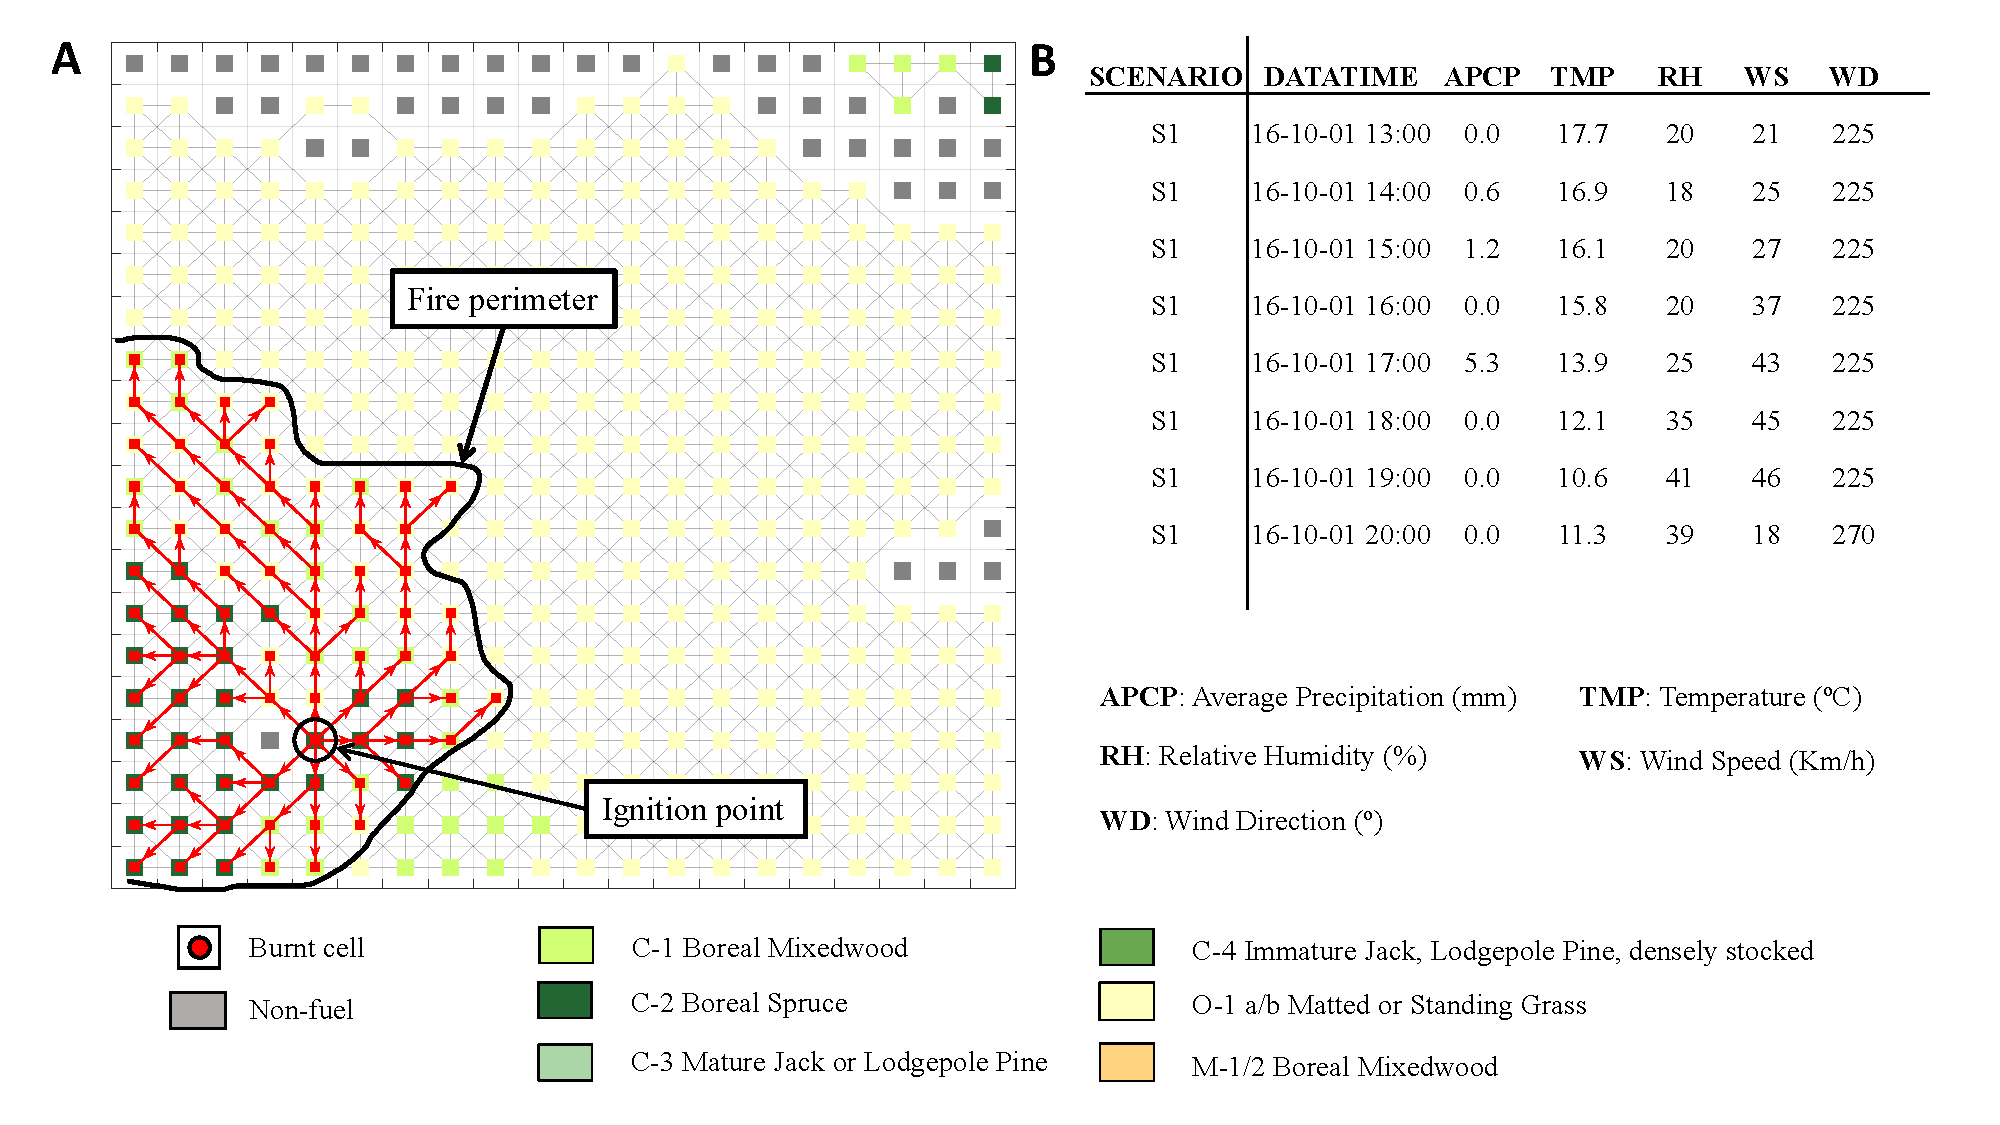
\includegraphics[scale=.5]{fig/landscape.pdf}
\vspace{1ex}
\caption{\textbf{A}: Graph representation of the
landscape and an example wildfire;
\textbf{B}: Example of a fire-weather scenario.}
\label{fig:graphs_landscape}
\end{figure}

\begin{figure}[htbp]
\centering
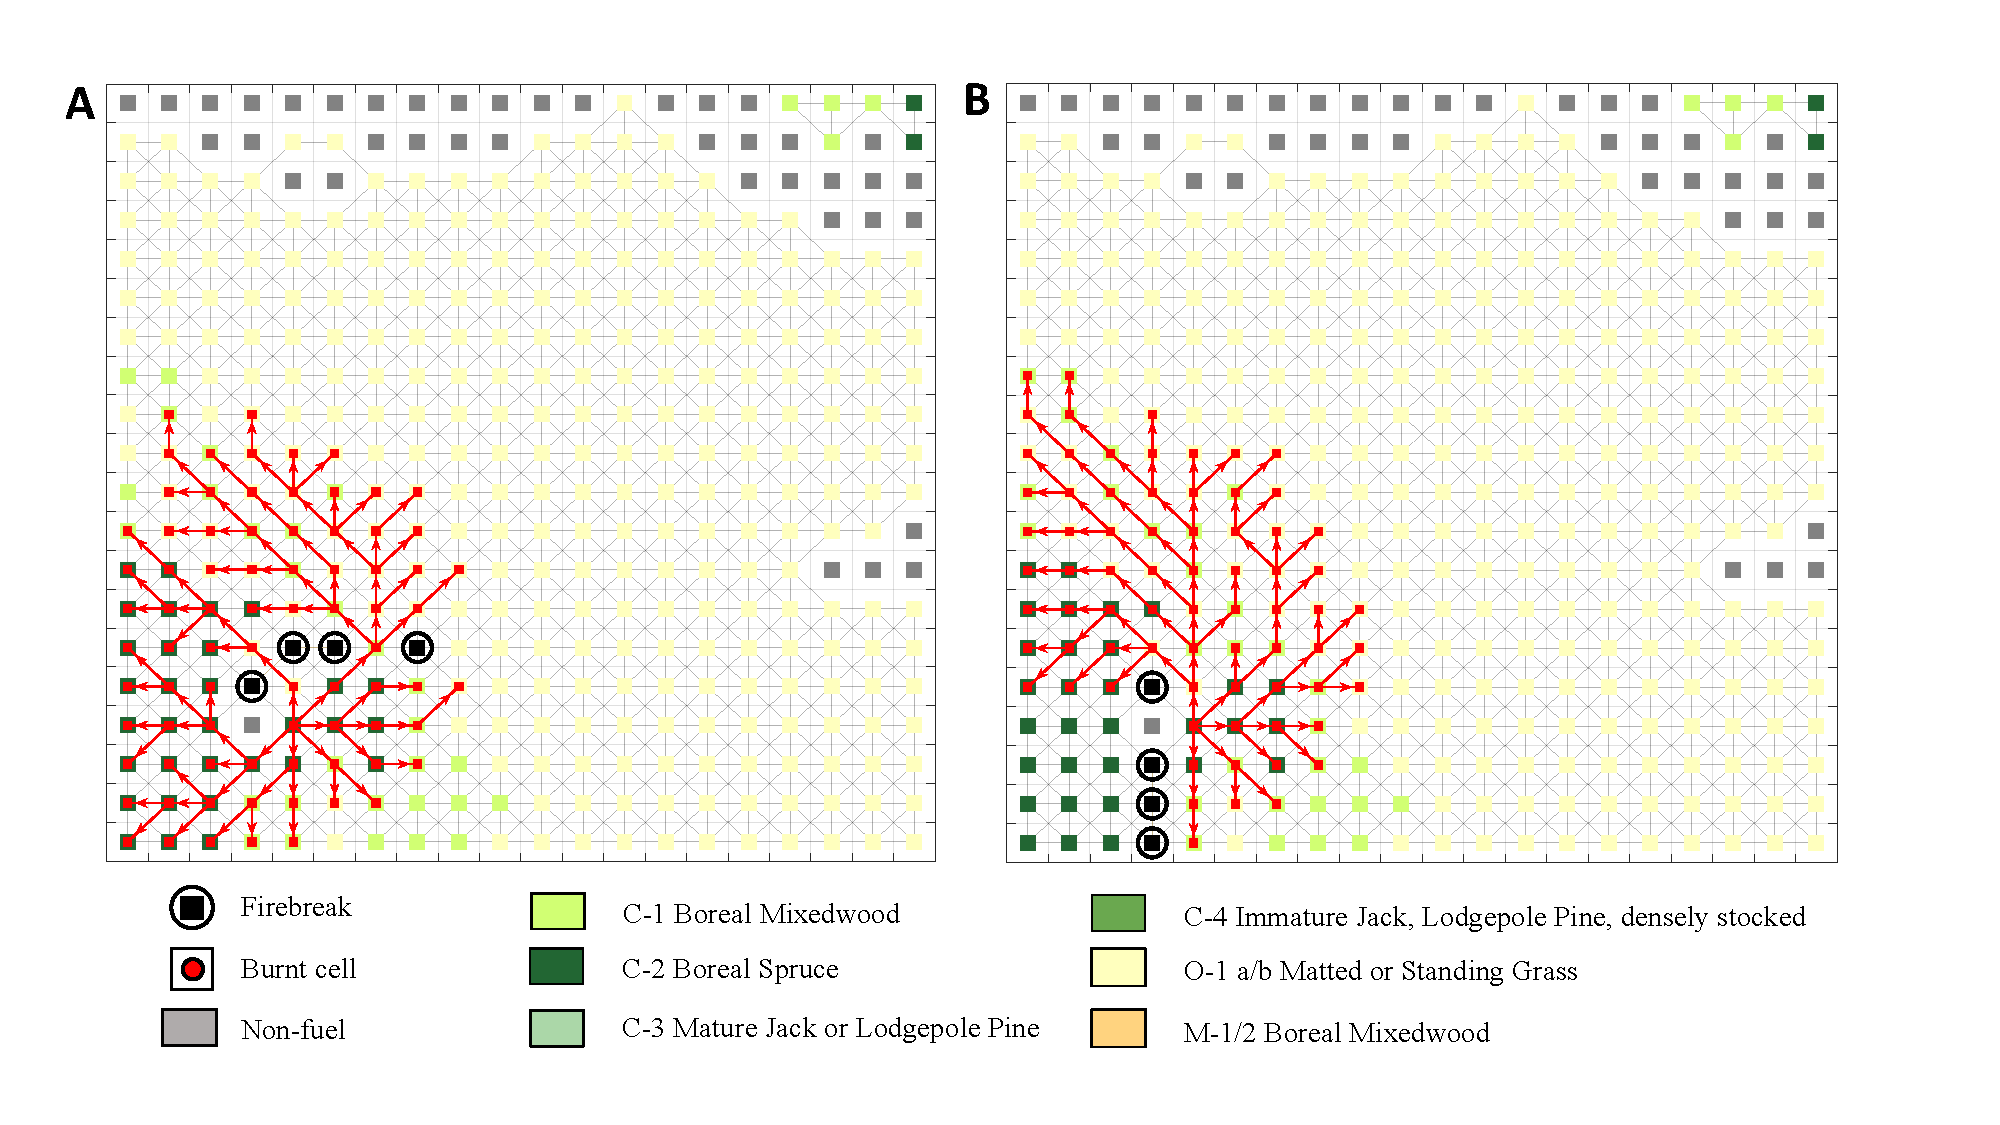
\includegraphics[scale=.5]{fig/firebreaks.pdf}
\vspace{1ex}
\caption{Comparison of two firebreak configurations
under the same wildfire scenario.
Configuration \textbf{B} prevents more cells
from burning than configuration \textbf{A}.}
\label{fig:graphs}
\end{figure}


\subsection{Conditional Value-at-Risk}

Minimizing expected wildfire loss does not necessarily
provide sufficient protection against adverse wildfire
scenarios. To account for the consequences of extreme
events, we consider Conditional Value-at-Risk (CVaR),
a risk measure that characterizes losses in the upper
tail of a probability distribution.

For a fixed firebreak configuration $\vb{y}$,
let $L_{\vb{y}}=L(\vb{y},\vb{w},\tau)$ denote
the corresponding random wildfire loss.
Its cumulative distribution function is
\begin{align}
F_{\vb{y}}(z)
=
\mathbb{P}
\left(
L_{\vb{y}}\leq z
\right).
\end{align}
For a confidence level $\beta\in(0,1)$,
Value-at-Risk is defined as
\begin{align}
\operatorname{VaR}_{\beta}(L_{\vb{y}})
=
\inf\left\{
z\in\mathbb{R}:
F_{\vb{y}}(z)\geq\beta
\right\}.
\end{align}
The corresponding CVaR is given by
\begin{align}
\operatorname{CVaR}_{\beta}(L_{\vb{y}})
=
\frac{1}{1-\beta}
\int_{\beta}^{1}
\operatorname{VaR}_{\gamma}(L_{\vb{y}})
\,d\gamma.
\end{align}
CVaR can therefore be interpreted as the average
loss in the worst $(1-\beta)$ proportion of
wildfire outcomes.

Following \citet{rockafellar2000optimization},
CVaR admits the equivalent representation
\begin{equation}
\label{CVaR_Formula}
\operatorname{CVaR}_{\beta}(L_{\vb{y}})
=
\min_{\varphi\in\mathbb{R}}
\left\{
\varphi+
\frac{1}{1-\beta}
\mathbb{E}_{\tau}
\left[
\left(
L(\vb{y},\vb{w},\tau)-\varphi
\right)^+
\right]
\right\},
\end{equation}
where $(a)^+=\max\{a,0\}$ and $\varphi$
represents a loss threshold. This representation
allows CVaR to be incorporated into a stochastic
optimization model through linear auxiliary
variables and constraints.

For a finite scenario set $\Omega$, with
scenario probabilities $\rho^\omega\geq 0$
satisfying
$\sum_{\omega\in\Omega}\rho^\omega=1$,
the expectation in
\eqref{CVaR_Formula} is replaced by a
probability-weighted sum of scenario losses.
For an equally weighted sample,
$\rho^\omega=1/n$ for every
$\omega\in\Omega$.


    


\section{Two-stage stochastic programming formulation}
\label{s:general-model}

We formulate the FPP as a two-stage stochastic mixed-integer
linear program. In the first stage, firebreak locations are
selected before wildfire uncertainty is realized. In the
second stage, the resulting wildfire losses are evaluated
across a finite set of propagation scenarios.

Let $\Omega$ denote the set of wildfire scenarios, with
probabilities $\rho^\omega \geq 0$ satisfying
$\sum_{\omega\in\Omega}\rho^\omega=1$.
Each scenario $\omega\in\Omega$ is represented by a
directed propagation graph
$\mathcal{T}^\omega=(\mathcal{V}^\omega,
\mathcal{E}^\omega)$ and an ignition node
$v(\omega)\in\mathcal{V}^\omega$. The first-stage binary variables $y_v$ determine the
firebreak placement, as introduced in
Section~\ref{sec2}. For each scenario $\omega\in\Omega$,
we introduce binary variables $x_v^\omega$, equal to
one if cell $v\in\mathcal{V}^\omega$ burns under the
selected firebreak configuration, and zero otherwise.
The corresponding scenario loss is represented by
$\sum_{v\in\mathcal{V}^\omega}w_vx_v^\omega$. To account for both average and adverse wildfire outcomes,
we consider an objective combining expected loss and
Conditional Value-at-Risk (CVaR). The parameter
$\lambda\in[0,1]$ controls the relative importance
of these criteria, while $\beta\in(0,1)$ denotes
the CVaR confidence level. Following the representation
introduced in Section~\ref{sec2}, we introduce a loss
threshold $\varphi$ and nonnegative auxiliary variables
$\eta^\omega$ to linearize the CVaR term.

The resulting formulation is given by
\allowdisplaybreaks{
\begin{subequations}
\label{m:fpp}
\begin{align}
\underset{\vb{x},\vb{y},\varphi,\vb{\eta}}
{\text{minimize}}
\quad &
\lambda
\sum_{\omega\in\Omega}\rho^\omega
\sum_{v\in\mathcal{V}^\omega}w_vx_v^\omega
+
(1-\lambda)
\left(
\varphi+
\frac{1}{1-\beta}
\sum_{\omega\in\Omega}\rho^\omega\eta^\omega
\right)
\label{fo:min_expected4}
\end{align}
\begin{align}
\text{subject to:}\quad
&
\sum_{v\in\mathcal{V}}y_v
\leq\alpha|\mathcal{V}|,
&&
\label{c:capacity}
\\
&
x_{v(\omega)}^\omega=1,
&&\forall\omega\in\Omega,
\label{c:ignition}
\\
&
x_v^\omega\leq x_u^\omega+y_u,
&&\forall\omega\in\Omega,\;
(v,u)\in\mathcal{E}^\omega,
\label{c:spread}
\\
&
\sum_{v\in\mathcal{V}^\omega}w_vx_v^\omega
-\varphi\leq\eta^\omega,
&&\forall\omega\in\Omega,
\label{c:cvar_linearization}
\\
&
\eta^\omega\geq0,
&&\forall\omega\in\Omega,
\label{c:eta}
\\
&
\varphi\geq0,
&&
\\
&
y_v\in\{0,1\},
&&\forall v\in\mathcal{V},
\nonumber
\\
&
x_v^\omega\in\{0,1\},
&&\forall\omega\in\Omega,\;
v\in\mathcal{V}^\omega.
\label{c:variables}
\end{align}
\end{subequations}
}
The objective function \eqref{fo:min_expected4} minimizes
a convex combination of expected wildfire loss and CVaR.
When $\lambda=1$, the formulation minimizes expected loss,
corresponding to a risk-neutral objective. Conversely,
$\lambda=0$ yields pure CVaR minimization, while intermediate
values balance expected losses and exposure to adverse
wildfire scenarios. Constraint \eqref{c:capacity} limits the number of cells
allocated to firebreaks. Constraints \eqref{c:ignition}
and \eqref{c:spread} represent wildfire propagation
under each scenario. The ignition node is always considered
burned. For every directed arc
$(v,u)\in\mathcal{E}^\omega$, constraint
\eqref{c:spread} requires cell $u$ to burn whenever
fire reaches cell $v$, unless a firebreak is placed
at $u$. Thus, a selected firebreak blocks incoming
propagation into the corresponding cell. By convention,
the ignition cell remains burned even if it is
selected for treatment. Constraints \eqref{c:cvar_linearization} and
\eqref{c:eta} impose
$\eta^\omega\geq
\max\{
0,\,
\sum_{v\in\mathcal{V}^\omega}
w_vx_v^\omega-\varphi
\}$. When $\lambda<1$, these variables attain their
corresponding positive-part values at optimality
for scenarios with positive probability.
Finally, constraint \eqref{c:variables} imposes
the integrality of the placement and burn variables.

An important property of formulation~\eqref{m:fpp}
is that the integrality constraints on the second-stage burn variables can be relaxed without
changing the optimal objective value. This property,
established in the following proposition, provides
the basis for the linear programming subproblems
used in the decomposition framework developed
in Section~\ref{sec:branch_benders}.

\begin{proposition}
\label{prop:integrality_recourse}
For any feasible first-stage decision
$\vb{y}\in\mathbb{Y}$, the second-stage problem
admits an optimal solution with binary burn
variables. Consequently, relaxing
$x_v^\omega\in\{0,1\}$ to
$0\leq x_v^\omega\leq1$
for all $v\in\mathcal{V}^\omega$ and
$\omega\in\Omega$ does not change the
optimal objective value of
formulation~\eqref{m:fpp}.
\end{proposition}

\begin{proof}
Consider any feasible binary firebreak configuration
$\vb{y}\in\mathbb{Y}$. For each scenario
$\omega\in\Omega$, define
$\hat{x}_v^\omega=1$ if $v$ is reachable from
the ignition node $v(\omega)$ through a directed
path containing no selected non-ignition
firebreaks, and $\hat{x}_v^\omega=0$ otherwise. By construction,
$\hat{x}_{v(\omega)}^\omega=1$.
Moreover, for every arc
$(v,u)\in\mathcal{E}^\omega$, if
$\hat{x}_v^\omega=1$ and $y_u=0$, then
$\hat{x}_u^\omega=1$. Hence,
$\hat{\vb{x}}^\omega$ satisfies the
propagation constraints.

Now consider any feasible fractional solution
$\vb{x}^\omega\in[0,1]^{|\mathcal{V}^\omega|}$.
Since $x_{v(\omega)}^\omega=1$, the propagation
constraints imply that $x_v^\omega=1$
for every cell reachable from the ignition
through a path containing no selected
non-ignition firebreaks. Therefore, 
$\hat{x}_v^\omega\leq x_v^\omega,
\qquad
\forall v\in\mathcal{V}^\omega$. 
Since $w_v\geq0$, it follows that $\sum_{v\in\mathcal{V}^\omega}
w_v\hat{x}_v^\omega
\leq
\sum_{v\in\mathcal{V}^\omega}
w_vx_v^\omega$. Thus, replacing $\vb{x}^\omega$ by
$\hat{\vb{x}}^\omega$ in every scenario
cannot increase any scenario loss.
The replacement preserves feasibility,
including the CVaR linearization
constraints, and cannot increase the
objective value for any $\lambda\in[0,1]$. Consequently, every optimal solution
of the formulation with relaxed burn
variables admits a binary counterpart
with the same optimal objective value.
\end{proof}


\section{Branch-and-Benders and graph-based inequalities}
\label{sec:branch_benders}

The extensive formulation (8) introduces burn variables for every cell and wildfire scenario. To address the resulting computational challenges, we develop a Branch-and-Benders decomposition framework that retains the first-stage firebreak placement decisions in a master problem and approximates the scenario-dependent recourse costs. We further strengthen the master problem through graph-based valid inequalities that provide lower bounds on scenario losses. Unless otherwise stated, the theoretical results in this section apply to general finite directed propagation graphs, without requiring a tree structure.

\subsection{Exact decomposition}
\label{subsec:exact_decomposition}

The proposed decomposition separates the first-stage firebreak placement decisions from the scenario-dependent wildfire propagation decisions. For each scenario $\omega \in \Omega$, we introduce a nonnegative master variable $\theta^\omega$ representing a lower approximation of the corresponding second-stage recourse cost. The variables $\varphi$ and $\eta^\omega$ retain their definitions from formulation~\eqref{m:fpp}, representing the CVaR loss threshold and the scenario-specific excess loss, respectively. The resulting master problem is formulated as follows:
\begin{equation}
\label{m:fpp_bd}
\begin{aligned}
\underset{\vb{y},\vb{\theta},\varphi,\vb{\eta}}{\text{minimize}}
\quad &
\lambda \sum_{\omega \in \Omega} \rho^\omega \theta^\omega
+ (1-\lambda)
\left(
\varphi + \frac{1}{1-\beta}
\sum_{\omega \in \Omega} \rho^\omega \eta^\omega
\right)\\
\text{subject to:}\quad
& \vb{y} \in \mathbb{Y},\\
& \eta^\omega \geq \theta^\omega - \varphi
&& \forall \omega \in \Omega,\\
& \eta^\omega \geq 0,\quad \theta^\omega \geq 0
&& \forall \omega \in \Omega,\\
& \varphi \geq 0.
\end{aligned}
\end{equation}
The constraints $\theta^\omega \geq Q^\omega(\vb{y})$, where $Q^\omega(\vb{y})$ denotes the optimal second-stage loss under scenario $\omega$, are progressively enforced through Benders optimality cuts.

For a given first-stage solution $\bar{\vb{y}} \in [0,1]^{|\mathcal{V}|}$, we formulate the scenario subproblem following the variable-copy approach of \citet{rahmaniani2020benders} as follows:
\begin{equation}
\label{m:fpp_sp}
\begin{aligned}
Q^\omega(\bar{\vb{y}})
= \underset{\vb{x}^\omega,\tilde{\vb{y}}^\omega}{\text{minimize}}
\quad &
\sum_{v \in \mathcal{V}^\omega} w_v x_v^\omega\\
\text{subject to:}\quad
& x_{v(\omega)}^\omega = 1,\\
& x_v^\omega \leq x_u^\omega + \tilde{y}_u^\omega
&& \forall v \in \mathcal{V}^\omega,\;
u \in \delta_+^\omega(v),\\
& \tilde{y}_v^\omega = \bar{y}_v
&& \forall v \in \mathcal{V},\\
& 0 \leq x_v^\omega \leq 1
&& \forall v \in \mathcal{V}^\omega,\\
& 0 \leq \tilde{y}_v^\omega \leq 1
&& \forall v \in \mathcal{V}.
\end{aligned}
\end{equation}
Here, $\tilde{y}_v^\omega$ denotes a scenario-specific copy of the first-stage variable $y_v$, linked to the master solution through the fixing constraints $\tilde{y}_v^\omega=\bar{y}_v$. As established in Proposition~\ref{prop:integrality_recourse}, the linear programming subproblem \eqref{m:fpp_sp} yields the exact scenario loss for any feasible binary firebreak placement. For fractional first-stage solutions, it defines the LP recourse function used to generate Benders optimality cuts.


Let $\pi_v^\omega$ denote the dual multiplier associated with the fixing constraint $\tilde{y}_v^\omega=\bar{y}_v$. By linear programming duality, the solution of the scenario subproblem yields the following Benders optimality cut:
\begin{equation}
\label{c:benders_optimality}
\theta^\omega \geq Q^\omega(\bar{\vb{y}})
+ \sum_{v \in \mathcal{V}}
\pi_v^\omega (y_v-\bar{y}_v),
\qquad \forall \omega \in \Omega.
\end{equation}
These cuts provide globally valid affine lower bounds on the recourse function and are tight at the evaluated solution $\bar{\vb{y}}$.

One limitation of the Branch-and-Benders framework is that weak initial approximations of the scenario recourse costs may require numerous subproblem evaluations and Benders cuts, leading to slow convergence. To address this limitation, we investigate graph-based valid inequalities that exploit the structure of wildfire propagation to strengthen the master problem's recourse estimates $\theta^\omega$. 

\subsection{Valid inequalities from downstream sets}
\label{subsec:coverage_inequalities}

A lower bound on the scenario recourse cost can be obtained by estimating the maximum protection that a firebreak configuration could provide. The underlying idea is to identify the cells potentially protected by each firebreak and subtract their associated values from the wildfire loss without intervention. Since this estimate may overstate the actual protection, the resulting expression provides a lower bound on the recourse cost.

For each scenario $\omega \in \Omega$, let $R^\omega(\vb{y})$ denote the set of cells reachable from the ignition node $v(\omega)$ under a binary firebreak configuration $\vb{y}$. In particular, $R^\omega(\vb{0})$ represents the cells burned in the absence of firebreaks. For each $v \in R^\omega(\vb{0}) \setminus \{v(\omega)\}$, we define its downstream set as
\begin{equation}
\label{eq:downstream_set}
D^\omega(v) =
\left\{
k \in R^\omega(\vb{0}) :
\text{there exists a directed path from } v
\text{ to } k \text{ in } \mathcal{T}^\omega
\right\},
\end{equation}
where each such cell belongs to its own downstream set. For all other cells, we set $D^\omega(v)=\emptyset$. In particular, the ignition node is excluded because it always burns and its selection as a firebreak does not prevent further propagation.

Treating a cell $v$ may prevent fire from reaching some or all of the cells in $D^\omega(v)$. However, alternative propagation paths may allow these cells to burn despite the treatment. Consequently, $\sum_{k \in D^\omega(v)} w_k$ represents an upper bound on the reduction in wildfire loss attributable to treating $v$.

When several firebreaks are selected, their downstream sets may overlap, causing the potential protection of individual cells to be counted multiple times. To account for this overlap, we consider subsets of the cells reachable without intervention and construct lower bounds on their contribution to the scenario loss.

For each scenario $\omega \in \Omega$, let $U \subseteq R^\omega(\vb{0})$ be any subset of these cells. By restricting the wildfire loss to $U$ and subtracting the potential protection associated with the selected firebreaks, we obtain the following family of inequalities:
\begin{equation}
\label{eq:coverage_projected}
\theta^\omega \geq
\sum_{k \in U} w_k
-
\sum_{v \in \mathcal{V}}
\left(
\sum_{k \in D^\omega(v) \cap U} w_k
\right)y_v,
\quad
\forall U \subseteq R^\omega(\vb{0}),\;
\omega \in \Omega.
\end{equation}
These inequalities estimate the remaining wildfire loss within $U$ by subtracting an upper bound on the protection attributable to the selected firebreaks. Their validity follows from the propagation constraints.

\begin{proposition}
\label{prop:coverage_validity}
For every scenario $\omega \in \Omega$, inequalities
\eqref{eq:coverage_projected} provide valid lower bounds
on $Q^\omega(\vb{y})$ for all
$\vb{y} \in [0,1]^{|\mathcal{V}|}$.
\end{proposition}

\begin{proof}
Consider any $\vb{y} \in [0,1]^{|\mathcal{V}|}$,
$U \subseteq R^\omega(\vb{0})$, and $k \in U$.
Since $k$ is reachable from the ignition node without
intervention, there exists a directed path
$p=(v(\omega)=v_0,v_1,\ldots,v_m=k)$ connecting these
nodes.

Summing the propagation constraints along this path yields  $x_k^\omega \geq
1-\sum_{j=1}^{m}y_{v_j}$. Every non-ignition node $v_j$ on this path satisfies
$k \in D^\omega(v_j)$. Since $y_v \geq 0$, we obtain $x_k^\omega \geq
1-\sum_{\substack{v \in \mathcal{V}: k \in D^\omega(v)}}y_v$. The nonnegativity of the burn variables and cell weights implies
\begin{align*}
Q^\omega(\vb{y})
&\geq
\sum_{k \in U}w_k x_k^\omega
\nonumber
&\geq
\sum_{k \in U}w_k
\left(
1-
\sum_{\substack{v \in \mathcal{V}:\\
k \in D^\omega(v)}}y_v
\right)
\nonumber
&=
\sum_{k \in U}w_k
-
\sum_{v \in \mathcal{V}}
\left(
\sum_{k \in D^\omega(v)\cap U}w_k
\right)y_v.
\end{align*}
Therefore, inequalities \eqref{eq:coverage_projected}
are valid.
\end{proof}

An important particular case is obtained by choosing $U=R^\omega(\vb{0})$ in \eqref{eq:coverage_projected}, yielding
\begin{equation}
\label{eq:llbi}
\theta^\omega \geq
\sum_{k \in R^\omega(\vb{0})} w_k
-
\sum_{v \in \mathcal{V}}
\left(
\sum_{k \in D^\omega(v)} w_k
\right)y_v,
\qquad \forall \omega \in \Omega.
\end{equation}
Inequality \eqref{eq:llbi} estimates the remaining wildfire loss by subtracting the potential protection associated with each selected firebreak over the entire set of cells reachable without intervention. However, overlapping downstream sets may cause the protection value of a cell to be subtracted multiple times, weakening the resulting lower bound.

The family \eqref{eq:coverage_projected} addresses this limitation by allowing cells to be excluded when their inclusion would weaken the inequality. Although this family contains exponentially many inequalities, its strongest member at a given $\bar{\vb{y}} \in [0,1]^{|\mathcal{V}|}$ can be identified directly. Indeed, each cell $k$ contributes $w_k(1- \sum_{\substack{v \in \mathcal{V}: k \in D^\omega(v)}}\bar{y}_v$ to the right-hand side of \eqref{eq:coverage_projected}. Since $w_k \geq 0$, a maximizing subset is therefore given by  $U = \{
k \in R^\omega(\vb{0}) :
\sum_{\substack{v \in \mathcal{V}: k \in D^\omega(v)}}\bar{y}_v < 1
\}$, with either choice permitted when equality holds.

Since \eqref{eq:llbi} is a particular member of \eqref{eq:coverage_projected}, the complete family provides a lower bound at least as strong as \eqref{eq:llbi}. By selecting cells according to their cumulative potential protection, these inequalities can yield tighter approximations of the scenario recourse cost.

\subsection{Valid inequalities from propagation paths}
\label{subsec:path_inequalities}

The inequalities in \eqref{eq:coverage_projected} estimate the potential
protection provided by firebreaks through their downstream sets. A
complementary approach exploits the propagation paths connecting the
ignition node to each cell. The underlying observation is that a cell
must burn whenever at least one path from the ignition remains
unblocked. Consequently, each propagation path provides a lower bound
on the burning of its destination cell, which can be used to construct
lower bounds on the scenario recourse cost.

For each scenario $\omega \in \Omega$ and
$k \in R^\omega(\vb{0})$, let $\mathcal{P}_k^\omega$
denote the set of directed simple paths from the ignition node
$v(\omega)$ to $k$ in $\mathcal{T}^\omega$.
For a path $p \in \mathcal{P}_k^\omega$, let $V(p)$
denote its set of vertices. The ignition node is excluded from
firebreak protection along the path, whereas the destination cell
is included whenever it differs from the ignition.
In particular, the trivial path from $v(\omega)$ to itself
contains no firebreak locations.

Consider any subset $U \subseteq R^\omega(\vb{0})$ and
select a path $p_k \in \mathcal{P}_k^\omega$ for each
$k \in U$. If none of the non-ignition cells along $p_k$
is protected, fire necessarily reaches $k$.
More generally, the propagation constraints imply that
the burning of $k$ is bounded below by one minus the
sum of the firebreak decisions along the selected path.
Aggregating these bounds over $U$ yields the following
family of inequalities:
\begin{equation}
\label{eq:path-proj}
\theta^\omega \geq
\sum_{k \in U} w_k
-
\sum_{k \in U} w_k
\sum_{v \in V(p_k)\setminus\{v(\omega)\}} y_v,
\quad
\begin{aligned}
&\forall U \subseteq R^\omega(\vb{0}), 
&\forall p_k \in \mathcal{P}_k^\omega,\; k \in U,
&\forall \omega \in \Omega.
\end{aligned}
\end{equation}
Each inequality estimates the remaining wildfire loss over
$U$ using one propagation path per cell. Unlike
\eqref{eq:coverage_projected}, which bounds the potential
protection associated with downstream sets, these
inequalities directly account for the firebreak locations
that can interrupt a particular route of propagation.

\begin{proposition}
\label{prop:path}
For every scenario $\omega \in \Omega$, inequalities
\eqref{eq:path-proj} provide valid lower bounds on
$Q^\omega(\vb{y})$ for all
$\vb{y} \in [0,1]^{|\mathcal{V}|}$.
\end{proposition}

\begin{proof}
Consider any $\vb{y} \in [0,1]^{|\mathcal{V}|}$,
$U \subseteq R^\omega(\vb{0})$, and a selection
$p_k \in \mathcal{P}_k^\omega$ for every $k \in U$.

For each selected path
$p_k=(v(\omega)=v_0,v_1,\ldots,v_m=k)$,
summing the propagation constraints along its arcs gives $x_k^\omega \geq
1-\sum_{j=1}^{m}y_{v_j}$. For the trivial path to the ignition node, this
inequality reduces to $x_{v(\omega)}^\omega \geq 1$.

Since the burn variables and cell weights are nonnegative,
every feasible second-stage solution satisfies
\begin{align*}
\sum_{k \in \mathcal{V}^\omega}w_k x_k^\omega
\geq
\sum_{k \in U}w_k x_k^\omega
\nonumber
\geq
\sum_{k \in U}w_k
-
\sum_{k \in U}w_k
\sum_{v \in V(p_k)\setminus\{v(\omega)\}}y_v.
\end{align*}
Taking the minimum over feasible second-stage solutions
establishes the validity of \eqref{eq:path-proj}.
\end{proof}

Note that when all directed simple paths are considered, the complete family \eqref{eq:path-proj} describes the epigraph of $Q^\omega(\vb{y})$ over
$\vb{y} \in [0,1]^{|\mathcal{V}|}$.  To see this, let $d_k^\omega(\vb{y})$ denote the minimum
sum of firebreak decisions along any directed path from
$v(\omega)$ to $k$, excluding the ignition node.
For a fixed $\vb{y}$, the strongest inequality in
\eqref{eq:path-proj} is obtained by selecting a
minimum-cost path for each cell satisfying
$d_k^\omega(\vb{y})<1$ and omitting the remaining cells.
Its right-hand side is
\[
\sum_{k \in R^\omega(\vb{0})}
w_k\max\{0,1-d_k^\omega(\vb{y})\}.
\]
This value is attained by the scenario recourse problem.
Indeed, setting
$x_k^\omega=\max\{0,1-d_k^\omega(\vb{y})\}$
for every $k \in R^\omega(\vb{0})$, and zero otherwise,
satisfies the propagation constraints.
This follows from the shortest-path property
$d_v^\omega(\vb{y})\leq d_u^\omega(\vb{y})+y_v$
for every propagation arc $(u,v)$ with
$v\neq v(\omega)$ and reachable tail $u$.
Hence, the maximum right-hand side of
\eqref{eq:path-proj} coincides with
$Q^\omega(\vb{y})$.

The inequalities in \eqref{eq:path-proj} are closely related to the
path-based Benders optimality cuts developed by
\citet{taninmics2024benders} for the Measure-Based Spread Minimization
Problem (MBSMP), which minimizes the expected spread of contagion
in stochastic directed networks by deactivating groups of labeled arcs.

A correspondence between the two problems can be established by
assigning label $j$ to every arc $(i,j)\in\mathcal{E}^{\omega}$.
Deactivating label $j$ then removes all incoming arcs to node $j$,
reproducing the effect of placing a firebreak at that node.
In particular, for $\lambda=1$, unit cell weights, equally
probable scenarios, and a common ignition node, the two formulations
coincide on the same collection of scenario graphs when the MBSMP
has unit label costs and budget
$B=\lfloor\alpha|\mathcal{V}|\rfloor$. Our formulation further accommodates scenario-dependent ignition
locations, heterogeneous cell weights, and CVaR-based risk preferences,
while representing wildfire propagation through simulated scenarios
rather than the independent-cascade model considered in the MBSMP.
The inequalities in \eqref{eq:path-proj} extend the corresponding
path-based construction to this setting.


\subsection{Separation of valid inequalities}
\label{subsec:separation}

The inequalities introduced in Sections~\ref{subsec:coverage_inequalities}
and~\ref{subsec:path_inequalities} are used to strengthen the scenario recourse estimates in the Branch-and-Benders master problem. Inequality \eqref{eq:llbi} can be added directly, since its coefficients depend only on the scenario graph. In contrast, \eqref{eq:coverage_projected} and \eqref{eq:path-proj} define exponential families, making their explicit inclusion impractical. We therefore develop separation procedures that generate selected inequalities at the current master solution.

For a given scenario $\omega\in\Omega$, let
$(\bar{\vb{y}},\bar\theta^\omega)$ denote the current solution of the master relaxation. Separation consists of identifying an inequality whose right-hand side exceeds $\bar\theta^\omega$ by more than a prescribed tolerance $\varepsilon>0$.

For \eqref{eq:coverage_projected}, the right-hand side can be
maximized by selecting the cells whose cumulative potential
protection is less than their contribution to the wildfire loss.
More precisely, each cell $k$ contributes positively when
$\sum_{\substack{v\in\mathcal V: k\in D^\omega(v)}}\bar y_v<1$. Thus, the strongest inequality at $\bar{\vb{y}}$ can be
identified without enumerating the subsets of
$R^\omega(\vb{0})$. Algorithm~\ref{alg:separate_coverage}
summarizes this procedure.
\allowdisplaybreaks{
\begin{algorithm}[htbp]
\caption{Separation of \eqref{eq:coverage_projected}}
\label{alg:separate_coverage}
\begin{algorithmic}[1]
\Require Scenario $\omega$, master solution
$(\bar{\vb{y}},\bar\theta^\omega)$,
downstream sets $D^\omega(v)$, tolerance $\varepsilon$
\Ensure A violated inequality or $\emptyset$

\State $U\gets\emptyset$

\For{$k\in R^\omega(\vb{0})$}
    \State $s_k\gets
    \displaystyle\sum_{\substack{v\in\mathcal V:\\
    k\in D^\omega(v)}}\bar y_v$
    \If{$s_k<1$}
        \State $U\gets U\cup\{k\}$
    \EndIf
\EndFor

\State $a^\omega\gets\displaystyle\sum_{k\in U}w_k$

\For{$v\in\mathcal V$}
    \State $c_v^\omega\gets
    \displaystyle\sum_{k\in D^\omega(v)\cap U}w_k$
\EndFor

\If{$a^\omega-
\displaystyle\sum_{v\in\mathcal V}c_v^\omega\bar y_v
>\bar\theta^\omega+\varepsilon$}
    \State \Return
    $\displaystyle\theta^\omega\geq
    a^\omega-\sum_{v\in\mathcal V}c_v^\omega y_v$
\EndIf

\State \Return $\emptyset$
\end{algorithmic}
\end{algorithm}
}

Separation of \eqref{eq:path-proj} requires identifying a
propagation path for each cell. Since the number of directed
simple paths may grow exponentially with the graph size,
we restrict the enumeration to at most $P_{\max}$ paths per
destination cell.

The paths are enumerated using depth-first search (DFS)
on the scenario graph, independently of the current
firebreak configuration. Paths containing the same set
of candidate firebreak locations are considered equivalent,
since they produce identical contributions to
\eqref{eq:path-proj}.

For a given $\bar{\vb{y}}$, the procedure selects the
minimum-cost path among those enumerated for each cell,
where the cost of a path is the sum of the firebreak
variables along its non-ignition vertices.
A cell contributes to the resulting inequality only if
this minimum cost is strictly less than one. Algorithm~\ref{alg:separate_paths} describes the separation
procedure.

\allowdisplaybreaks{
\begin{algorithm}[htbp]
\caption{Separation of \eqref{eq:path-proj}}
\label{alg:separate_paths}
\begin{algorithmic}[1]
\Require Scenario $\omega$, master solution
$(\bar{\vb{y}},\bar\theta^\omega)$,
path limit $P_{\max}$, tolerance $\varepsilon$
\Ensure A violated inequality or $\emptyset$

\State $U\gets\emptyset$
\State $a^\omega\gets0$
\State $c_v^\omega\gets0$ for all $v\in\mathcal V$

\For{$k\in R^\omega(\vb{0})$}

    \State Enumerate up to $P_{\max}$ directed simple paths
    from $v(\omega)$ to $k$ using DFS

    \State Let $\widehat{\mathcal P}_k^\omega$
    contain the enumerated paths after removing equivalent paths

    \State Select
    $p_k\in\displaystyle\arg\min_{p\in\widehat{\mathcal P}_k^\omega}
    \sum_{v\in V(p)\setminus\{v(\omega)\}}\bar y_v$

    \State $d_k\gets
    \displaystyle\sum_{v\in V(p_k)\setminus\{v(\omega)\}}\bar y_v$

    \If{$d_k<1$}
        \State $U\gets U\cup\{k\}$
        \State $a^\omega\gets a^\omega+w_k$

        \For{$v\in V(p_k)\setminus\{v(\omega)\}$}
            \State $c_v^\omega\gets c_v^\omega+w_k$
        \EndFor
    \EndIf

\EndFor

\If{$a^\omega-
\displaystyle\sum_{v\in\mathcal V}c_v^\omega\bar y_v
>\bar\theta^\omega+\varepsilon$}
    \State \Return
    $\displaystyle\theta^\omega\geq
    a^\omega-\sum_{v\in\mathcal V}c_v^\omega y_v$
\EndIf
\State \Return $\emptyset$
\end{algorithmic}
\end{algorithm}
}
The two procedures differ in the information used to
construct their inequalities. Algorithm~\ref{alg:separate_coverage}
uses the downstream sets of candidate firebreak locations
and identifies the strongest member of
\eqref{eq:coverage_projected} at the current solution.
Algorithm~\ref{alg:separate_paths}, instead, exploits
explicit propagation paths and identifies the strongest
member of \eqref{eq:path-proj} among the enumerated paths.
Restricting the path collection may weaken the resulting
lower bound but does not affect the validity of the
generated inequalities.

Both procedures are incorporated into the Branch-and-Benders framework through successive separation rounds at the root LP relaxation. At each round, the current solution is used to identify violated inequalities, which are added to the master problem before reoptimization. The process terminates when no further inequalities are generated or when the
prescribed separation limits are reached. The inequalities generated during this phase remain in the master problem throughout the subsequent branch-and-bound search. They complement the Benders optimality cuts obtained from the scenario subproblems, which continue to ensure the exact evaluation of integer candidate solutions.


\section{Computational experiments}\label{sec:computational}
This section evaluates the computational performance of the proposed Branch-and-Benders framework and the quality of the resulting firebreak placement decisions. We first describe the experimental setup and the benchmark algorithms. We then compare their computational performance across different scenario sample sizes, firebreak budgets, and risk preferences. Finally, we assess the out-of-sample performance and stability of the resulting firebreak placements using independent wildfire scenarios.

\subsection{Experimental setup}
\label{sec:compared}

The computational experiments consider a forest area near Villarrica
Volcano in southern Chile, represented by a $20\times20$ grid comprising
400 cells. Wildfire scenarios are generated using the Cell2Fire simulator
\citep{pais2021cell2fire}, which simulates fire ignition and propagation
under different environmental conditions. Each simulation produces a
directed graph representing the spread of fire from its ignition point.
For optimization, these graphs are reduced using a shortest-path-based
procedure that represents propagation routes from the ignition to the
affected cells. The resulting graphs may contain multiple paths to the
same cell and are therefore not necessarily trees. Both the in-sample optimization and the out-of-sample evaluation use these reduced propagation graphs. All cell weights are set to $w_v=1$.

We consider three scenario sample sizes, $n\in\{100,200,400\}$, and
three firebreak intensities, $\alpha\in\{0.01,0.02,0.03\}$, corresponding
to budgets of 4, 8, and 12 cells, respectively. The risk-weighting
parameter takes values $\lambda\in\{0,0.5,1\}$, with CVaR confidence
level $\beta=0.9$. For each combination of scenario sample size, firebreak intensity, and risk-weighting parameter, 30 independent scenario samples are generated, yielding a total of $3\times3\times3\times30=810$ instances.

We compare the extensive mixed-integer linear programming formulation
with four variants of the proposed Branch-and-Benders decomposition and
a combinatorial Branch-and-Benders benchmark. All methods use CPLEX to solve the master mixed-integer
program. The four LP-based Branch-and-Benders variants
solve scenario linear programming subproblems, generating
Benders optimality cuts at integer candidate solutions
and additional LP-dual cuts at the root relaxation.
The combinatorial benchmark instead generates optimality
cuts without solving scenario LPs. The distinguishing
features of the methods are summarized in
Table~\ref{tab:methods}.

\begin{table}[htbp]
\centering
\normalfont
\caption{Optimization methods considered in the computational experiments.}
\label{tab:methods}
\begin{tabular}{p{0.14\linewidth}p{0.76\linewidth}}
\toprule
Method & Description \\
\midrule
MILP &
Extensive formulation
\eqref{fo:min_expected4}--\eqref{c:variables},
solved directly by CPLEX using sample average approximation (SAA).
\\

B\&B &
Standard Branch-and-Benders decomposition described in
Section~\ref{subsec:exact_decomposition}, without additional graph-based inequalities.
\\

B\&B-I &
B\&B strengthened with the static inequality \eqref{eq:llbi},
added to the initial master problem.
\\

B\&B-II &
B\&B strengthened with inequalities \eqref{eq:coverage_projected},
dynamically separated at the root relaxation.
\\

B\&B-III &
B\&B strengthened with inequalities \eqref{eq:path-proj},
dynamically separated at the root relaxation using bounded
depth-first search.
\\

CB\&B &
Combinatorial Branch-and-Benders approach adapted from
\citet{taninmics2024benders}, generating Benders cuts through
combinatorial procedures without solving scenario LPs.
\\
\bottomrule
\end{tabular}
\end{table}

All experiments were conducted using IBM ILOG CPLEX Optimization
Studio 22.1.1, with one thread, a time limit of 1,800 seconds, and
a relative MIP optimality gap tolerance of $10^{-3}$. Apart from these settings and the method-specific cut-generation procedures, default CPLEX parameters were retained. The source code implementing the proposed algorithms and computational experiments is publicly available at \url{https://github.com/FrancoQuezada/stochastic-firebreak-placement}.

Computational performance is assessed through solution times,
final optimality gaps, and the percentage of instances certified
optimal. Certification requires an \texttt{Optimal} solver status
and a final relative MIP gap not exceeding $10^{-3}$.
Reported runtime and gap statistics include all runs, including
those terminated at the time limit. Cumulative certification profiles are also used to compare the methods over time.

To evaluate solution quality, firebreak placements obtained with
B\&B-III are assessed on a common independent test set of 1,000
wildfire scenarios. This out-of-sample evaluation examines the
performance and stability of the resulting solutions across
different scenario sample sizes, firebreak intensities, and
risk preferences.


\subsection{Algorithmic performance}\label{sec:results}

Table~\ref{tab:new20-gaps-times} compares the six methods across the three risk-weighting settings. For each method and risk setting, the proportion of instances solved to optimality is calculated over 270 instances. Reported optimality gaps and solver times include both optimal and time-limited instances. 

\begin{table}[htbp]
    \centering
    \caption{Algorithmic performance on 270 instances per method and value of $\lambda$. Mean and maximum final gaps are reported in percent, and mean observed solver time in seconds.}
    \label{tab:new20-gaps-times}
\begin{tabular}{@{}clrrrr@{}}
\toprule
$\lambda$ & Method & Optimal (\%) & Mean gap (\%) & Max. gap (\%) & Mean time (s) \\
\midrule
\multirow{6}{*}{$1.0$}
 & MILP      & 100.0 & 0.01 & 0.10 & 178.4 \\
 & B\&B      & 65.2  & 3.57 & 16.11 & 748.6 \\
 & B\&B-I    & 64.1  & 3.77 & 16.50 & 774.4 \\
 & B\&B-II   & 95.6  & 0.11 & 1.59 & 203.2 \\
 & B\&B-III  & 100.0 & 0.05 & 0.10 & 71.3 \\
 & CB\&B     & 100.0 & 0.04 & 0.10 & 28.4 \\
\midrule
\multirow{6}{*}{$0.5$}
 & MILP      & 60.0 & 2.41 & 29.68 & 1071.8 \\
 & B\&B      & 38.9 & 7.07 & 21.72 & 1160.0 \\
 & B\&B-I    & 40.4 & 7.39 & 21.93 & 1139.2 \\
 & B\&B-II   & 65.2 & 1.29 & 10.12 & 825.2 \\
 & B\&B-III  & 87.8 & 0.39 & 4.64 & 461.1 \\
 & CB\&B     & 78.5 & 0.89 & 8.56 & 697.8 \\
\midrule
\multirow{6}{*}{$0.0$}
 & MILP      & 30.7 & 9.00 & 91.64 & 1452.7 \\
 & B\&B      & 37.8 & 9.36 & 27.04 & 1167.9 \\
 & B\&B-I    & 40.7 & 8.70 & 26.18 & 1125.9 \\
 & B\&B-II   & 50.0 & 3.09 & 11.60 & 1015.1 \\
 & B\&B-III  & 67.0 & 1.44 & 10.10 & 850.2 \\
 & CB\&B     & 53.3 & 3.02 & 18.08 & 1057.5 \\
\bottomrule
\end{tabular}
\end{table}

For expected-loss minimization ($\lambda=1$), MILP, B\&B-III, and CB\&B
solve all 270 instances to optimality. CB\&B achieves the lowest mean
computational time (28.4\,s), followed by B\&B-III (71.3\,s) and MILP
(178.4\,s). The advantage of CB\&B is consistent with its combinatorial
treatment of the scenario subproblems. For a fixed firebreak placement,
wildfire losses can be evaluated directly through graph reachability,
allowing CB\&B to generate optimality cuts without repeatedly solving
linear programming subproblems. Moreover, under expected-loss
minimization, scenario losses contribute linearly to the objective,
without the additional constraints associated with CVaR. This
combination may explain the efficiency of combinatorial cut generation
in this setting. As shown in Figure~\ref{fig:alg-expected},
CB\&B reaches a high proportion of optimal solutions considerably
earlier than the other methods. Nevertheless, B\&B-III also solves
every instance to optimality and requires less than half the average
computational time of MILP, demonstrating the effectiveness of the
proposed decomposition framework.

The comparison among the Branch-and-Benders variants highlights the
importance of strengthening the scenario recourse approximations.
Adding the static inequality \eqref{eq:llbi} in
B\&B-I provides limited and inconsistent improvements
over the standard B\&B approach. This limited effect is consistent
with the construction of the inequality, which may substantially
underestimate scenario losses when downstream sets overlap.
In contrast, B\&B-II dynamically separates
\eqref{eq:coverage_projected}, selecting the cells that contribute
positively to the lower bound at the current fractional solution.
This produces a more informative approximation of the recourse
function and substantially improves computational performance.
For instance, under expected loss, the proportion of optimal
solutions increases from 65.2\% with B\&B to 95.6\% with B\&B-II.

\begin{figure}[htbp]
\centering
\begin{subfigure}{0.7\linewidth}
    \centering
    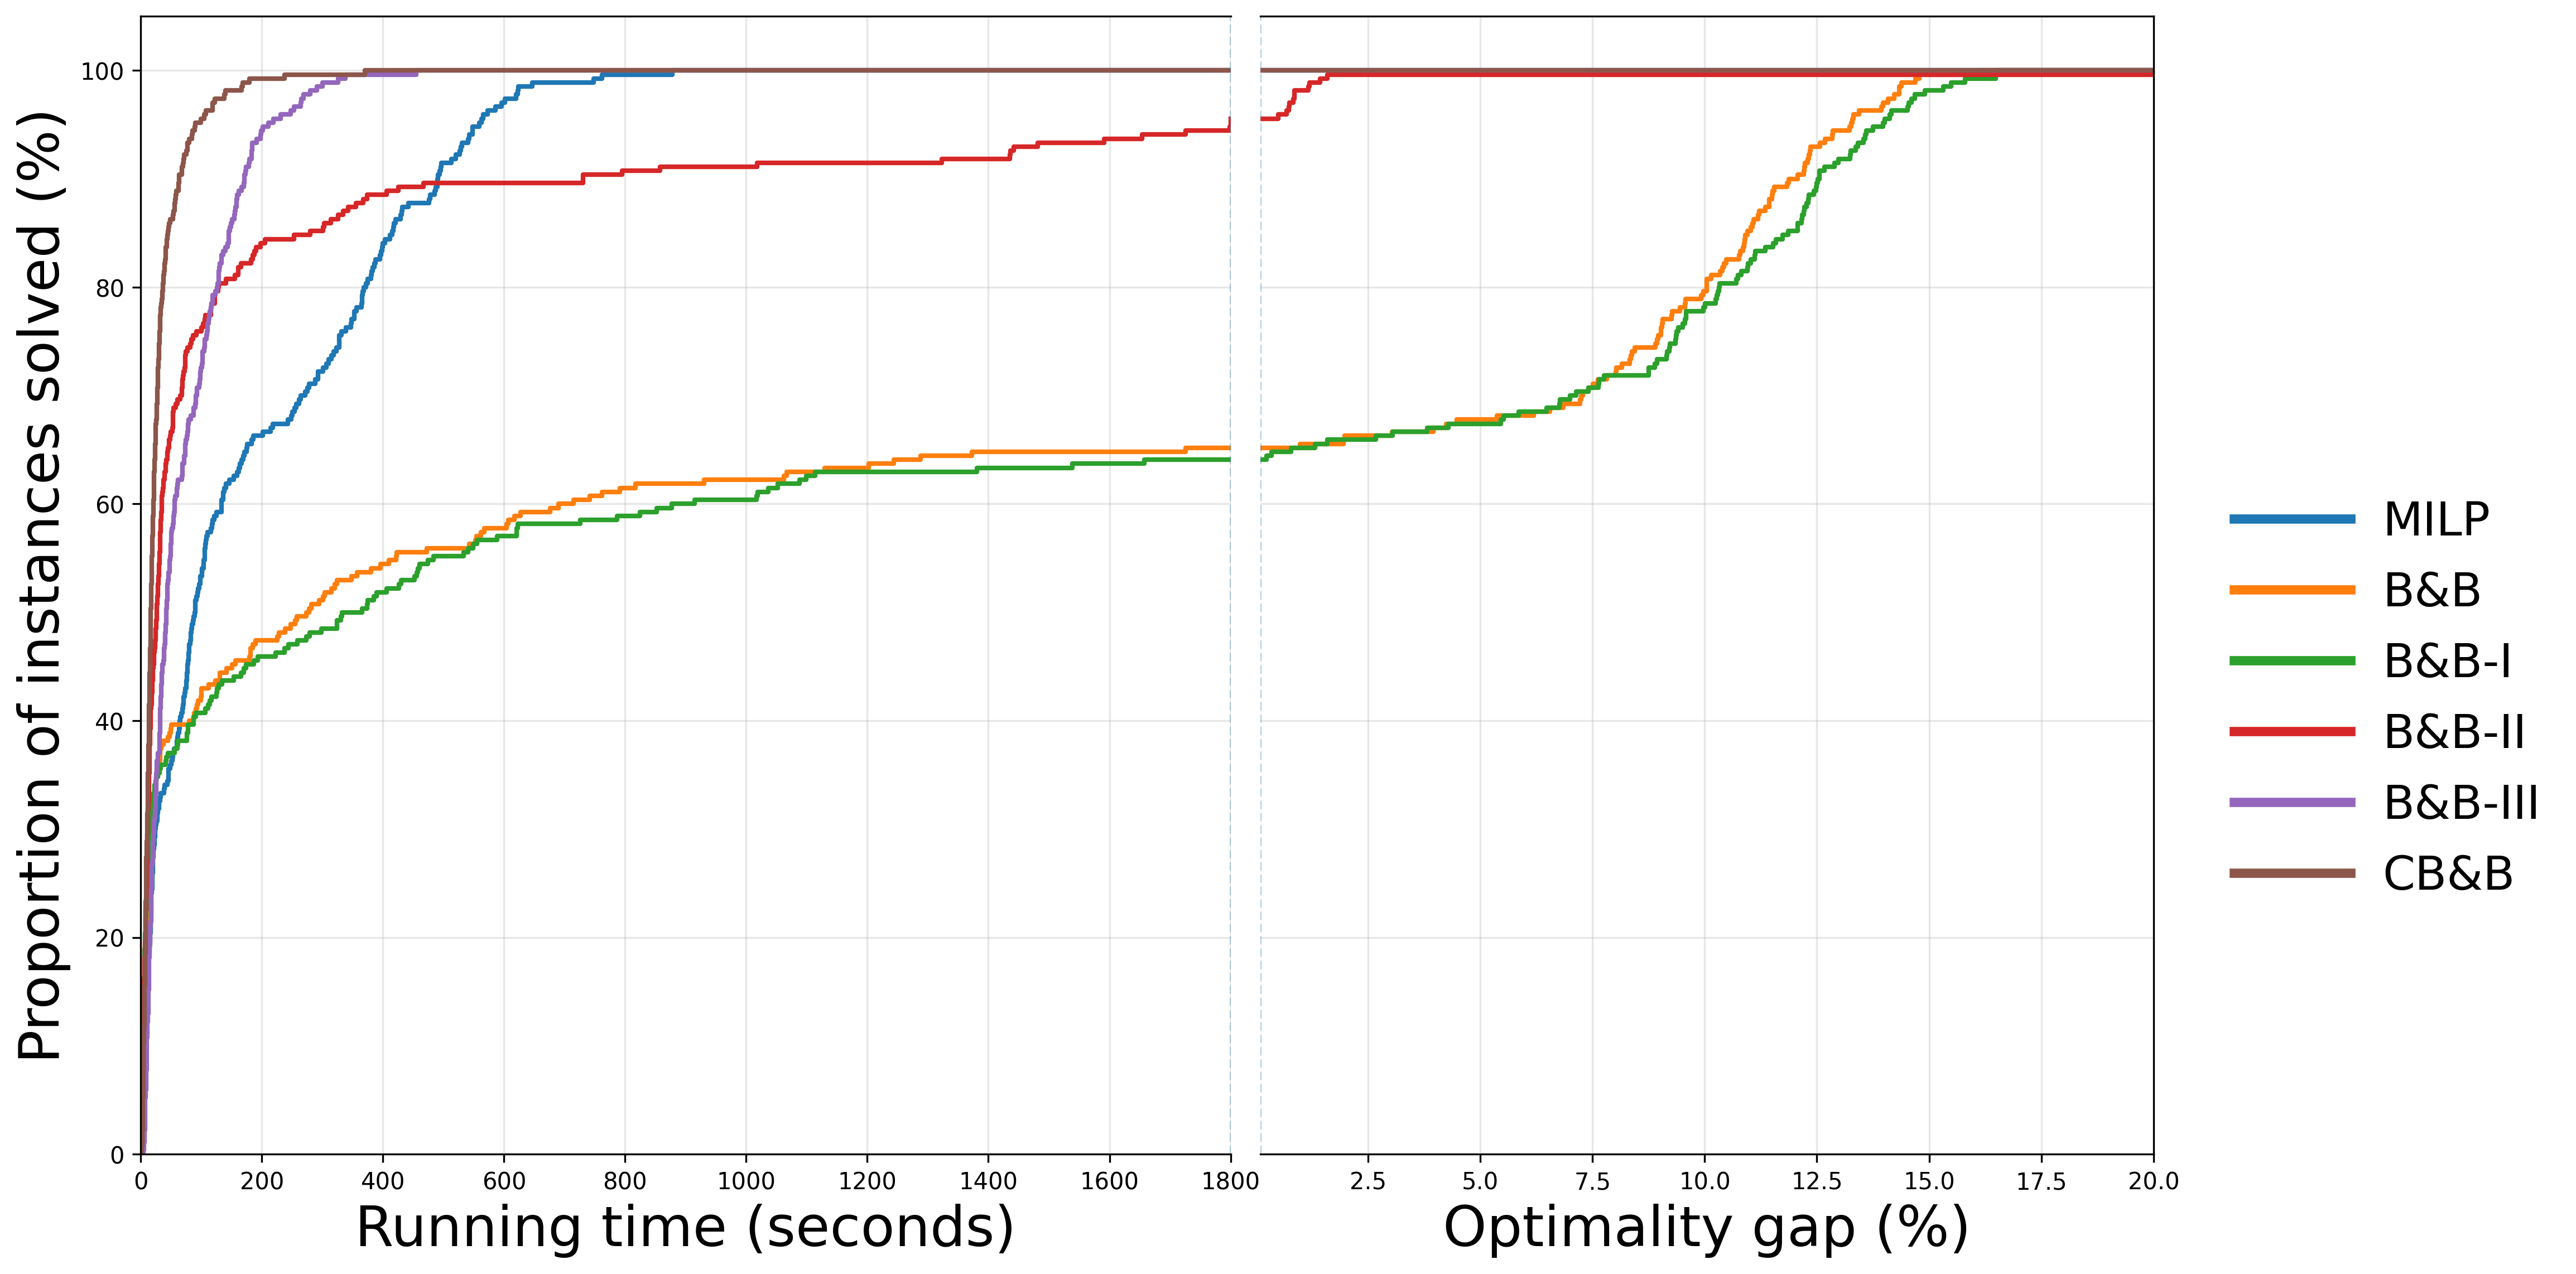
\includegraphics[width=\linewidth]
    {fig/performance_expected.png}
    \caption{Expected loss ($\lambda=1.0$).}
    \label{fig:alg-expected}
\end{subfigure}
\begin{subfigure}{0.7\linewidth}
    \centering
    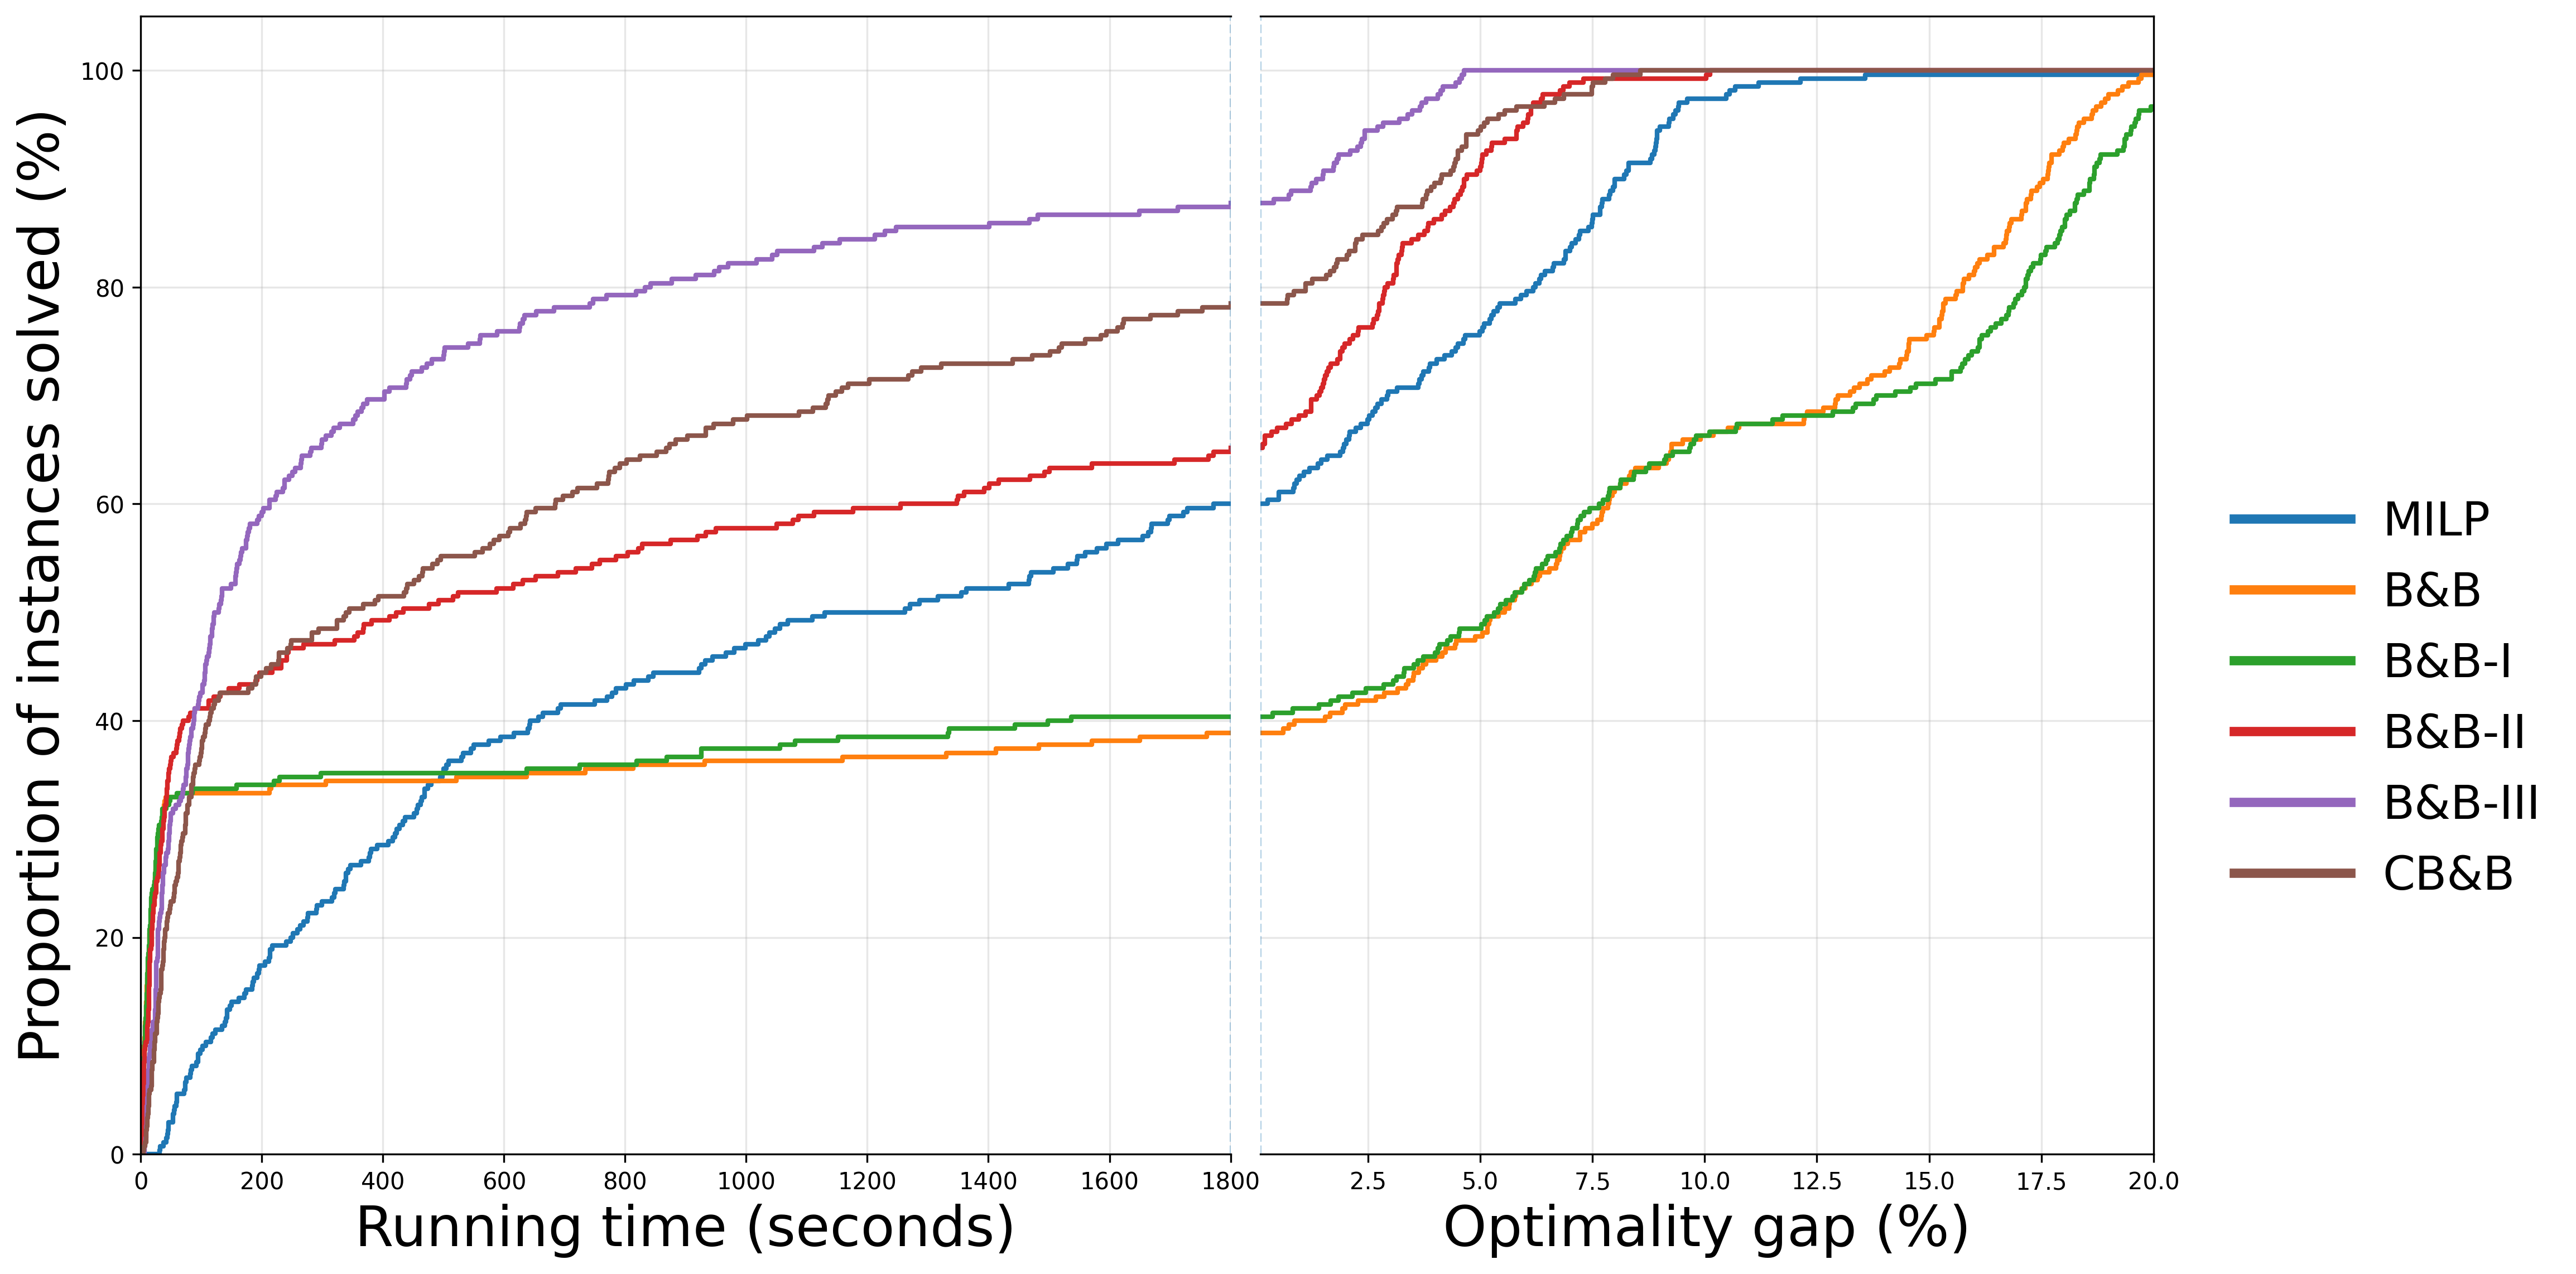
\includegraphics[width=\linewidth]
    {fig/performance_mean_cvar.png}
    \caption{Mean--CVaR ($\lambda=0.5$).}
    \label{fig:alg-mean-cvar}
\end{subfigure}
\begin{subfigure}{0.7\linewidth}
    \centering
    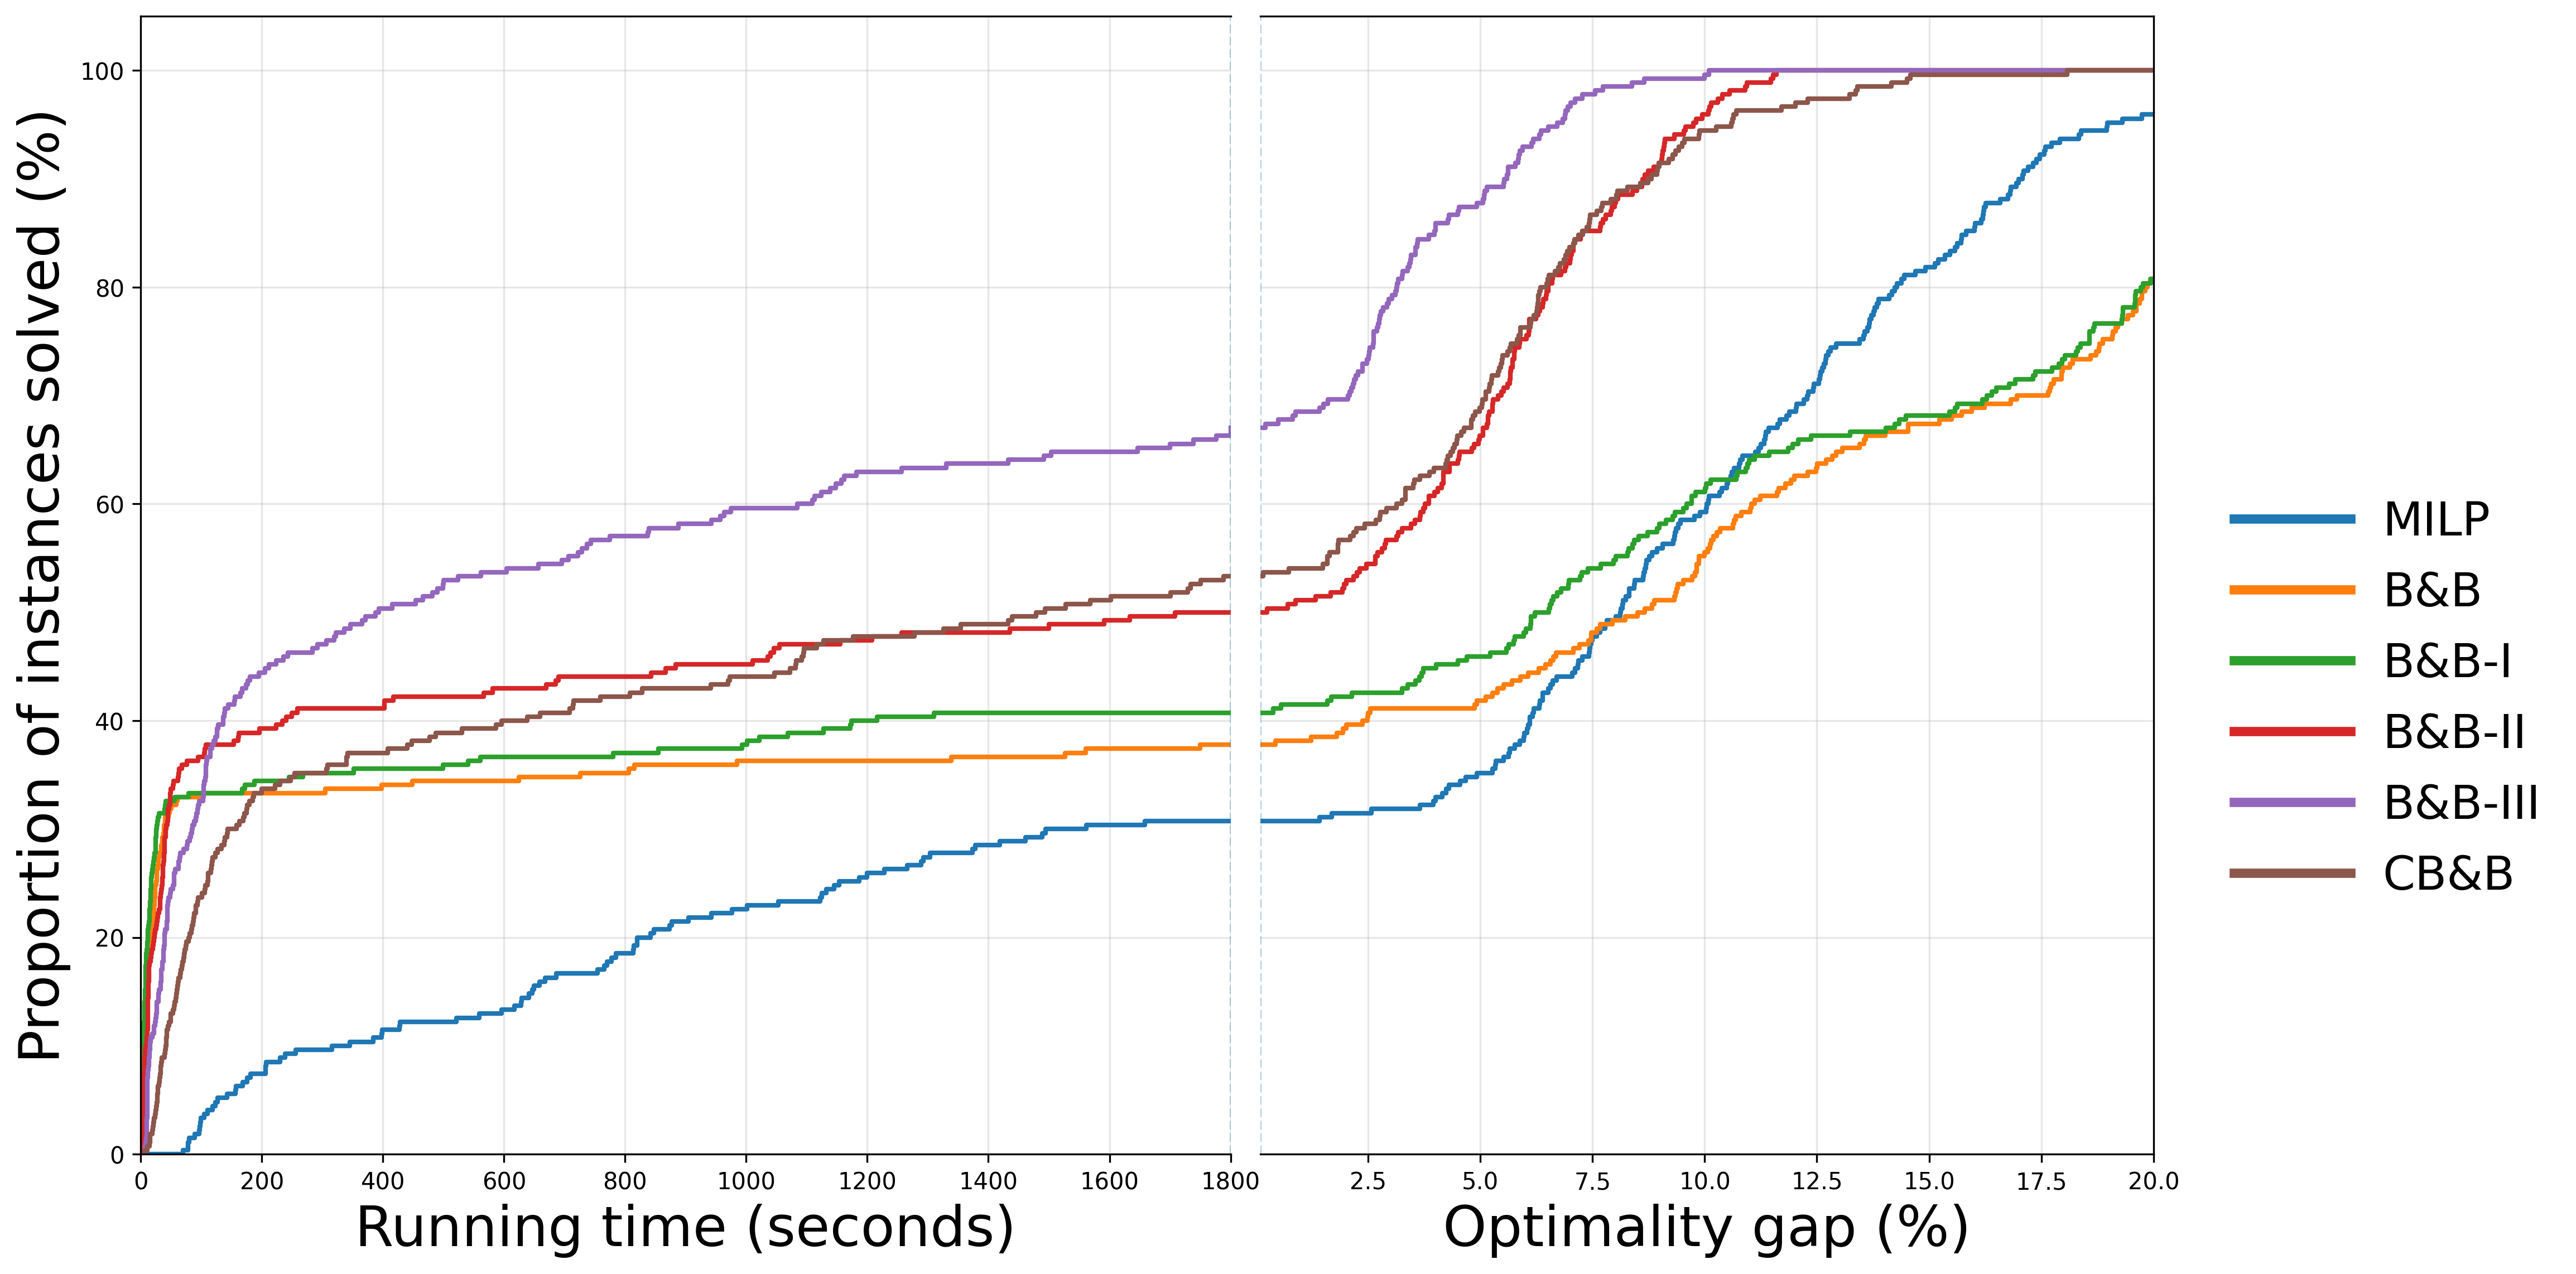
\includegraphics[width=\linewidth]    {fig/performance_cvar.png}
    \caption{CVaR ($\lambda=0.0$).}
    \label{fig:alg-cvar}
\end{subfigure}
\caption{Algorithmic performance under different risk preferences. Each plot shows the cumulative proportion of instances solved to optimality as a function of computational time (left) and the cumulative distribution of final relative optimality gaps (right). }
\label{fig:alg-performance}
\end{figure}

B\&B-III achieves further improvements by exploiting explicit propagation paths through inequalities \eqref{eq:path-proj}. Unlike downstream sets, which identify cells potentially protected by a firebreak, propagation paths provide information about the
alternative routes through which fire can reach a destination. This distinction is particularly relevant in graphs containing multiple propagation routes, where treating a cell does not necessarily prevent fire from reaching its downstream vertices. By accounting for these routes, the inequalities can provide tighter
lower bounds on scenario losses. Indeed, the complete family \eqref{eq:path-proj} characterizes the fractional recourse function, although the implemented separation procedure considers only a restricted collection of paths. The computational advantage of
B\&B-III is consistent with these stronger recourse approximations,
which can compensate for the additional effort required to
generate the inequalities.

The benefits of B\&B-III become particularly pronounced when tail risk is incorporated into the objective. Under CVaR minimization ($\lambda=0$), B\&B-III solves 67.0\% of instances to optimality, compared with 53.3\% for CB\&B and 50.0\% for B\&B-II. It also achieves the lowest mean optimality gap (1.44\%) and computational time (850.2\,s). Unlike expected-loss minimization, CVaR explicitly emphasizes scenarios whose losses exceed a common risk threshold. Consequently, inaccurate recourse approximations may underestimate both the losses in these scenarios and their contribution to the tail-risk objective. Strengthening the scenario-level lower bounds may therefore be especially valuable for the master problem. This provides a possible explanation for the improved relative performance of B\&B-III compared with CB\&B as risk aversion increases.

The performance profiles provide further evidence of this advantage. As shown in Figure~\ref{fig:alg-cvar}, B\&B-II initially solves a larger proportion of CVaR instances than B\&B-III, but the latter overtakes it as computational time increases. This behavior suggests that the additional separation effort of B\&B-III is compensated by its ability to solve more difficult instances. Furthermore, approximately 88\% of instances solved by B\&B-III finish with an optimality gap below 5\%, compared with 69\% for CB\&B. Thus, its advantage extends beyond the proportion of optimal solutions to the quality of the final optimality bounds.

A similar pattern emerges for the mean--CVaR setting
($\lambda=0.5$). B\&B-III solves 87.8\% of instances to optimality, compared with 78.5\% for CB\&B and 65.2\% for B\&B-II. It also reduces the mean computational time from 697.8\,s for CB\&B to 461.1\,s, while achieving a smaller mean final optimality gap (0.39\% versus 0.89\%). The corresponding distributions in Figure~\ref{fig:alg-mean-cvar} show that all B\&B-III instances finish with a gap below 5\%, including those not solved to optimality. These findings indicate that the benefits of the path-based inequalities persist when expected loss and tail risk are considered simultaneously.


The differences between methods become more pronounced as the firebreak budget increases. At $\alpha=0.03$, neither B\&B nor B\&B-I solves any of the 90 instances to optimality under any risk setting. In contrast, B\&B-III solves 90, 23, and 58 instances under expected loss, CVaR, and mean--CVaR, respectively. Larger budgets expand the set of feasible firebreak placements
and increase the interactions among potential protection decisions. Consequently, weak recourse approximations may leave a large number of promising but overly optimistic solutions in the master relaxation. The dynamically separated inequalities help reduce
this effect by exploiting the structure of wildfire propagation. The superior performance of B\&B-III at larger budgets suggests that explicit path information becomes particularly valuable as the placement decisions become more complex.


These results establish B\&B-III as the most effective variant of the proposed Branch-and-Benders framework. Its ability to exploit propagation-path information yields substantial improvements over the standard decomposition, particularly for larger firebreak budgets and risk-sensitive objectives. Although CB\&B remains the fastest method under expected-loss minimization, B\&B-III provides the strongest overall performance
when tail risk is considered. Accordingly, the subsequent
out-of-sample analysis uses B\&B-III to evaluate firebreak placements obtained through a common optimization procedure.

\subsection{Out-of-sample performance and solution stability}\label{sec:oos-stability}

We evaluate the B\&B-III placements obtained from 30 independent scenario
samples for each $(n,\alpha,\lambda)$ configuration on a common set of
1,000 independent wildfire scenarios. Their out-of-sample expected loss
$\widehat\mu(Y)$, CVaR $\widehat C_{0.9}(Y)$, and risk-weighted objective
$\widehat F_\lambda(Y)=\lambda\widehat\mu(Y)
+(1-\lambda)\widehat C_{0.9}(Y)$ are computed using the definitions
in Section~\ref{sec2}. 

To assess spatial stability, we use the Jaccard index
$J(Y_a,Y_b)=|Y_a\cap Y_b|/|Y_a\cup Y_b|$ and the optimal
matching distance $D(Y_a,Y_b)=\frac{1}{k}\min_{\pi\in S_k}
\sum_{i=1}^{k} \left\|\mathbf{p}_{u_i}-\mathbf{p}_{v_{\pi(i)}}\right\|_2,$ where $Y_a=\{u_1,\ldots,u_k\}$ and $Y_b=\{v_1,\ldots,v_k\}$
are placements of $k$ firebreak cells,
$\mathbf{p}_v=(r_v,c_v)$ denotes the row and column coordinates
of cell $v$, and $S_k$ denotes the set of all permutations
of $\{1,\ldots,k\}$. The distance measures the minimum
average separation between matched firebreak locations,
expressed in grid-cell widths. Both metrics are averaged over the
$\binom{30}{2}=435$ placement pairs within each configuration.
Table~\ref{tab:new20-oos-stability} reports held-out performance
and placement stability. All feasible placements are included,
even when optimality is not certified; the pairwise comparisons
are not independent replications.

\begin{table}[!htbp]
\centering
\caption{Out-of-sample performance and spatial stability of B\&B-III
placements from 30 independent solutions per configuration, evaluated
on a common 1,000-scenario test set. The columns $\widehat\mu$ and
$\widehat C_{0.9}$ give mean losses, while $\widehat F_\lambda$
reports its mean and sample standard deviation (SD).
Optimal (\%) is the percentage of solutions certified optimal.
$\overline J$ and $\overline D$ are the mean pairwise Jaccard
similarity and optimal matching distance, respectively;
the latter is expressed in grid-cell widths.}
\label{tab:new20-oos-stability}
\setlength{\tabcolsep}{4pt}
\renewcommand{\arraystretch}{1.07}
\begin{tabular}{@{}ccc r r r r r r@{}}
\toprule
$\lambda$ & $\alpha$ & $n$ & $\widehat\mu$ & $\widehat C_{0.9}$ & $\widehat F_\lambda$ (mean, SD) & Optimal (\%) & $\overline J$ & $\overline D$ \\
\midrule
\multirow{9}{*}{$1$} & \multirow{3}{*}{$0.01$} & 100 & 134.74 & 282.14 & 134.74 (1.58) & 100.0 & 0.37 & 2.09 \\
 &  & 200 & 133.59 & 284.95 & 133.59 (0.98) & 100.0 & 0.49 & 1.36 \\
 &  & 400 & 133.04 & 284.55 & 133.04 (0.56) & 100.0 & 0.61 & 1.06 \\
\cmidrule(l){2-9}
 & \multirow{3}{*}{$0.02$} & 100 & 93.46 & 209.20 & 93.46 (2.12) & 100.0 & 0.42 & 1.31 \\
 &  & 200 & 91.92 & 205.35 & 91.92 (1.30) & 100.0 & 0.54 & 0.87 \\
 &  & 400 & 91.59 & 204.48 & 91.59 (0.99) & 100.0 & 0.60 & 0.59 \\
\cmidrule(l){2-9}
 & \multirow{3}{*}{$0.03$} & 100 & 75.69 & 163.48 & 75.69 (1.47) & 100.0 & 0.40 & 1.69 \\
 &  & 200 & 74.28 & 155.66 & 74.28 (0.76) & 100.0 & 0.45 & 1.02 \\
 &  & 400 & 73.99 & 154.00 & 73.99 (0.58) & 100.0 & 0.49 & 0.83 \\
\midrule
\multirow{9}{*}{$0.5$} & \multirow{3}{*}{$0.01$} & 100 & 135.74 & 275.03 & 205.38 (3.62) & 100.0 & 0.34 & 1.91 \\
 &  & 200 & 135.64 & 269.72 & 202.68 (1.96) & 100.0 & 0.39 & 1.63 \\
 &  & 400 & 136.61 & 269.82 & 203.22 (2.17) & 100.0 & 0.41 & 1.82 \\
\cmidrule(l){2-9}
 & \multirow{3}{*}{$0.02$} & 100 & 98.21 & 201.16 & 149.68 (5.41) & 100.0 & 0.23 & 1.97 \\
 &  & 200 & 97.00 & 194.35 & 145.68 (2.36) & 100.0 & 0.31 & 1.51 \\
 &  & 400 & 95.66 & 191.47 & 143.56 (1.50) & 96.7 & 0.39 & 1.16 \\
\cmidrule(l){2-9}
 & \multirow{3}{*}{$0.03$} & 100 & 77.25 & 154.72 & 115.99 (3.49) & 96.7 & 0.35 & 1.49 \\
 &  & 200 & 75.79 & 150.50 & 113.14 (1.81) & 83.3 & 0.42 & 1.09 \\
 &  & 400 & 75.14 & 149.94 & 112.54 (1.46) & 13.3 & 0.47 & 1.02 \\
\midrule
\multirow{9}{*}{$0$} & \multirow{3}{*}{$0.01$} & 100 & 141.49 & 274.86 & 274.86 (9.22) & 100.0 & 0.25 & 2.52 \\
 &  & 200 & 139.83 & 269.70 & 269.70 (5.09) & 100.0 & 0.32 & 2.31 \\
 &  & 400 & 139.80 & 268.22 & 268.22 (2.38) & 100.0 & 0.49 & 1.70 \\
\cmidrule(l){2-9}
 & \multirow{3}{*}{$0.02$} & 100 & 100.69 & 199.19 & 199.19 (6.82) & 96.7 & 0.20 & 2.12 \\
 &  & 200 & 99.30 & 194.96 & 194.96 (5.04) & 100.0 & 0.28 & 1.73 \\
 &  & 400 & 98.87 & 192.63 & 192.63 (2.59) & 30.0 & 0.32 & 1.48 \\
\cmidrule(l){2-9}
 & \multirow{3}{*}{$0.03$} & 100 & 81.02 & 157.05 & 157.05 (7.80) & 56.7 & 0.30 & 1.70 \\
 &  & 200 & 78.90 & 148.98 & 148.98 (3.17) & 16.7 & 0.38 & 1.30 \\
 &  & 400 & 78.81 & 148.07 & 148.07 (2.47) & 3.3 & 0.43 & 1.20 \\
\bottomrule
\end{tabular}
\end{table}

Increasing the number of optimization scenarios generally improves
out-of-sample stability, with smaller gains beyond $n=200$.
At $\alpha=0.02$ and $\lambda=0.5$, the standard deviation of
the out-of-sample objective decreases from 5.41 to 1.50 as
$n$ increases from 100 to 400. Under CVaR minimization with
$\alpha=0.01$, the difference between mean in-sample and
out-of-sample CVaR decreases from 20.92 to 5.46, consistent
with reduced sampling optimism at larger sample sizes.

Larger scenario samples also lead to geographically more consistent
firebreak placements. Across all nine $(\alpha,\lambda)$ settings,
mean Jaccard similarity increases and mean optimal matching
distance decreases between $n=100$ and $n=400$. At $\alpha=0.02$,
expected-loss placements exhibit an increase in Jaccard similarity
from 0.42 to 0.60 and a decrease in matching distance from
1.31 to 0.59 grid-cell widths. The latter indicates that, after optimally matching the selected firebreak locations across independent solutions, their average geographical separation is less than one grid-cell width. Thus, placements that differ in
their exact selected cells can remain geographically close.
Risk-sensitive solutions exhibit greater spatial variability.
At $(n,\alpha)=(400,0.02)$, the mean matching distance is 1.16
for mean--CVaR and 1.48 for CVaR, compared with 0.59 under
expected-loss minimization. The persistence of spatial variation
alongside relatively stable out-of-sample losses suggests that
different placements can provide comparable protection.
Unresolved optimization gaps in the most challenging
risk-sensitive configurations may also contribute to this variation.

Risk preferences affect both out-of-sample losses and the locations
of selected firebreaks. At $(n,\alpha)=(200,0.02)$, the balanced
objective ($\lambda=0.5$) reduces CVaR by 5.4\% relative to
expected-loss minimization, at the cost of a 5.5\% increase in
expected loss. It also achieves tail-risk performance comparable
to pure CVaR minimization while retaining lower expected loss.
For corresponding scenario samples, balanced and CVaR placements
have a mean Jaccard similarity of 0.60 and matching distance of
0.83 grid-cell widths, compared with 0.32 and 2.21 between
expected-loss and CVaR placements. The balanced objective thus
produces firebreak locations geographically closer to those
favored by CVaR minimization.


\section{Conclusions}\label{sec:conclusions}

This paper addressed the stochastic firebreak placement problem through
a two-stage optimization formulation that integrates wildfire propagation
scenarios generated by Cell2Fire with a risk-weighted objective combining
expected loss and CVaR. We developed a Branch-and-Benders framework
that exploits the structure of directed propagation graphs to strengthen
the approximation of scenario recourse. In particular, we established
valid inequalities based on downstream sets and propagation paths.
The complete family of path-based inequalities characterizes the
fractional recourse function, providing a theoretical foundation for
the proposed strengthening strategies.

The computational experiments demonstrate the importance of exploiting
propagation structure within the decomposition framework. While the
initial static inequality provides limited improvements, dynamically
separated inequalities substantially enhance computational performance.
The path-based variant, B\&B-III, consistently outperforms the other
proposed variants, with particularly pronounced advantages under
risk-sensitive objectives. It solves all expected-loss instances to
optimality and achieves the highest proportion of optimal solutions
under CVaR (67.0\%) and mean--CVaR (87.8\%). Although the combinatorial
benchmark CB\&B is faster under expected-loss minimization, B\&B-III
performs better when tail risk is incorporated into the objective.
These findings highlight the computational value of propagation-path
information, particularly when accurate scenario recourse approximations
are important for representing adverse wildfire outcomes.

The out-of-sample analysis further demonstrates the benefits of
increasing the number of optimization scenarios. Larger samples generally
improve the quality of firebreak placements while reducing variability
in their performance on independent wildfire scenarios, although
the marginal improvements tend to diminish. Increasing the firebreak
budget also reduces wildfire losses, with decreasing marginal benefits
observed in the experiments. The risk-weighting parameter introduces
a meaningful trade-off between average protection and losses in severe
wildfire scenarios. Moreover, the Jaccard analysis reveals that spatial
similarity between independently obtained placements generally increases
with sample size and is higher under expected-loss minimization.
Nevertheless, relatively different firebreak configurations can achieve
similar out-of-sample performance, highlighting the distinction between
stability in decision quality and stability in selected locations.

These findings are subject to limitations associated with the
computational difficulty of larger risk-sensitive instances and the
use of reduced propagation graphs. Future research should investigate
more effective separation strategies for large-scale instances and
evaluate how the resulting placements perform on the corresponding
full propagation graphs. Extending the analysis to heterogeneous
cell values and environmental costs would also allow the optimization
to account more explicitly for ecological and socioeconomic priorities.
Overall, the results demonstrate that incorporating propagation-path
structure into stochastic decomposition provides an effective approach
to optimizing firebreak placement under uncertainty and risk aversion.


\section*{Acknowledgments}
This project has received funding from the European Union’s Horizon 2020 research and innovation program under grant agreement No 101037419 (\href{https://fire-res.eu}{FIRE-RES}) and the Complex Engineering Systems Institute (CONICYT-PIA-FB0816). Jaime Carrasco acknowledges the support of the ANID through funding Postdoctoral Fondecyt project No 3210311. Franco Quezada and Sebastián Dávila-Gálvez are grateful for the support of the National Agency for Research and Development (ANID) Chile through grant FONDECYT 11261130 and FONDECYT 11251766, respectively. Also, the authors gratefully acknowledge the research support provided by Dicyt project 062217DG, Vicerrector\'ia de Investigaci\'on, Desarrollo e Innovaci\'on, Universidad de Santiago de Chile. The authors gratefully acknowledge the contributions of David Palacios and Andr\'es Weintraub to earlier versions of this manuscript.

\bibliographystyle{itor}

\bibliography{references}


\end{document}
